%!TEX root = Thesis.tex

\chapter{Coordination Complexes with Palladium(0) and Platinum(0)}
\chaptermark{Palladium(0) and Platinum(0)}
\label{ch:platinum0}

Palladium and platinum are two rare elements of the so-called platinum group metals.  Although both palladium and platinum are rare elements, palladium is around three times more common than platinum with an abundance in the earth's crust of 0.015 and 0.005 ppm for palladium and platinum respectively.  Both palladium and platinum find uses in their elemental form in jewellery, most commonly as alloys with gold.  Palladium and platinum both find use as heterogeneous catalysts: large amounts of both metals are used in catalytic converters in cars to oxidise the unburned hydrocarbons and carbon monoxide that can be produced \emph{via} incomplete combustion.  Platinum also finds use as a metal in the electronics industry and as platinum crucibles.  Both of these applications rely on the high chemical and thermal resistance of platinum, particularly in the case of platinum crucibles which are frequently used to dissolve mineral samples using aggressive reagents such as hydrofluoric acid.  Indeed metallic platinum is so inert that an alloy of 90\%{} platinum and 10\%{} iridium (w/w) is used as the material for the international prototype kilogram, the mass of which defines the kilogram unit.  

\fixme{this needs citations}

Coordination complexes of palladium and platinum are used extensively.  Perhaps the most well-known platinum complex is \ce{[Pt(NH3)2Cl2]} (cisplatin).  Cisplatin, distributed under the trade name Platinol is a widely used chemotherapeutic which is used in conjunction with other therapies for the treatment of various cancers, most commonly tumours including sarcomas, carcinomas and lymphomas.  A further two platinum complexes (carboplatin and oxaliplatin) have been approved for use in chemotherapy worldwide with other complexes approved in select countries.\cite{Wilson2013}

Palladium complexes are some of the most commonly used coordination complexes in homogeneous catalysis, finding use in a wide-range of reactions including cross-coupling, allylic alkylation and various carbonylation reactions among many others, typically forming C-C, C-N and C-O bonds.\cite{Klingensmith2006}  These transformations are highly important for industrial processes and laboratory scale total-synthesis.  These catalytic reactions are thought to involve palladium in the 0 and +2 oxidation states.  Palladium is commonly used due to its balance of reactivity and stability, which is important for catalysts to have high \glspl{TOF} and \glspl{TON}.  This high reactivity can make palladium complexes and catalytic processes difficult to study. Platinum complexes are typically more inert than their corresponding palladium analogues to processes such as ligand exchange and redox changes.  The spin active isotope platinum-195 (34\% abundant) can result in platinum coupling in the NMR spectra the coupling constants of which, can lead to additional information regarding the geometry and bonding in the complex.  Platinum and palladium are otherwise very similar metals which makes the additional insight gained from platinum models of value when examining similar chemistry with palladium.  

Prior to the start of this work four studies had been published investigating the catalytic activity of \tBuxantphos{}.\cite{Mispelaere2005, Dongol2007, Ohshima2009, Cabello2007}  Two of these studies investigated the catalytic activity of \tBuxantphos{} palladium systems and one investigated platinum systems.  In all cases the little to no reactivity was observed with \tBuxantphos{} systems while the corresponding \Phxantphos{} reactions gave 40 - 99\% conversions.  This suggests differences in the coordination chemistry of the two ligands towards palladium and platinum.  However, no studies have investigated the coordination chemistry of \tBuxantphos{} with either palladium or platinum, in an attempt to explain the different activities.  A crystal structure of [Pd(\tBuxantphos)\ce{Cl2}] was reported to the \gls{CCDC} in 2011 which shows a bite-angle of 152.827\degrees{} compared to the 100.606 and 100.916\degrees{} for [Pd(\Phxantphos)\ce{Cl2}] with different solvates.  The difference in the bite-angles and geometries of the complexes that form may explain the difference in the catalytic reactivity of the complexes.  

Since the start of this work five further papers have been published investigating the catalytic activity of palladium complexes with \tBuxantphos{}.\cite{Ashcroft2013, Behr2013, Friis2014, Dang2013, Liu2013c}  In the palladium-catalysed Suzuki cross-coupling and the hydroesterification of methyl oleate little activity was observed with \tBuxantphos{} while the \Phxantphos{} complexes gave high yields.\cite{Ashcroft2013, Behr2013}  However, in the N-alkylation of amines with primary and secondary alcohols, the \tBuxantphos{} system was more active than the \Phxantphos{} system, with \tBuxantphos showing near quantitative conversion at 100\degC{} while the \Phxantphos{} system gave only 63\% conversion at 110\degC.  Similarly the methylation of alkynyl C-H bonds with dimethyl sulfonium ylides using \tBuxantphos{} went to 46\% conversion while \Phxantphos{} gave only 15\%.\cite{Liu2013c}  A palladium complex with a monodentate xantphos ligand was tested in the aminocarbonylation of hetero-aryl bromides, and showed no reactivity with \tBuxantphos{} while \Phxantphos gave a 92\% isolated yield.\cite{Friis2014}  Together these studies support the premise that the coordination chemistry of \tBuxantphos{} and \Phxantphos{} are distinct, likely as a result of the changes in the bite-angles and steric bulk between the ligands.  However, no research into this area has yet been reported. 

While the coordination chemistry of \Phxantphos{} on palladium has been the subject of a number of different studies, little research into the coordination chemistry of the \Phxantphos{} on platinum, particularly platinum(0), has been reported.\cite{Zuideveld2002, Raebiger2004, Bakhmutov2012, Miedaner2004, Klingensmith2006, Petocz2004, Yin2002}  The main focus of this chapter is investigation into the coordination chemistry of the three \tBuxantphos{} ligands with a range of  platinum and palladium(0) precursors.  Some reactivity of the resulting complexes towards small molecules is also presented.  A brief investigation into the coordination chemistry of \Phthixantphos{} with platinum(0) will also be presented for comparative purposes.  The subsequent chapter will address the coordination chemistry of the \tBuxantphos{} ligands with platinum and palladium(II) starting materials.  

%======================================================================

\section{Reactions of \Phthixantphos{} with Platinum(0) Precursors}

An equimolar ratio of the \Phthixantphos{} and tris-(norbornene)platinum \fixme{define nb} were combined in \ce{C6D6} the reaction immediately forms two products and does not progress further.  The \phosphorus{} NMR spectrum shows one sharp peak at 20.0 ppm (\JPtP~=~3470 Hz, 39.6\%) and one system with two overlapping broad singlets ranging from 0 to -10 ppm (60.4\%).  The platinum-phosphorus coupling constant on the sharp signal is consistent with a mono-alkene complex such as, [Pt(nb)(\Phxantphos)].  The \proton{} NMR spectrum showed a number of aromatic signals together with peaks that can be ascribed to tris-(norbornene)platinum and uncoordinated norbornene, as well as new alkyl and alkene proton signals.  This suggests that the complex appearing at 20.0 ppm in the \phosphorus{} NMR spectrum is [Pt(nb)(\Phxantphos)], while the other complex has more than one molecule of \Phxantphos{} per platinum atom.  Attempts to synthesis [Pt(nb)(\Phxantphos)] exclusively were unsuccessful, as were attempts to isolate the complex from the product mixture.  As such, this species was not characterised fully.  However, the \proton{} NMR spectrum does show a peak at \fixme{value, around 2.55 ppm} which appears as a broad triplet, consistent with a coordinated alkene.  

The reaction between \Phthixantphos{} and tris-(norbornene)platinum was repeated using a 2:1 ratio of diphosphine:platinum.  In this case only the broad species between 0 and -10 ppm was observed by \phosphorus{} NMR.  Upon removal of the displaced norbornene from the system, under reduced pressure, the \proton{} NMR spectrum displayed only aromatic signals.  This indicates that the complex formed under these conditions does not contain any alkene or alkyl ligand nor is there any evidence for uncoordinated \Phthixantphos{} ligand.  From this data we can propose [Pt(\Phthixantphos\ce{)2]} as the product from this reaction (Scheme \ref{scheme:PtSPh2}).

\begin{scheme}[ht]
\begin{center}
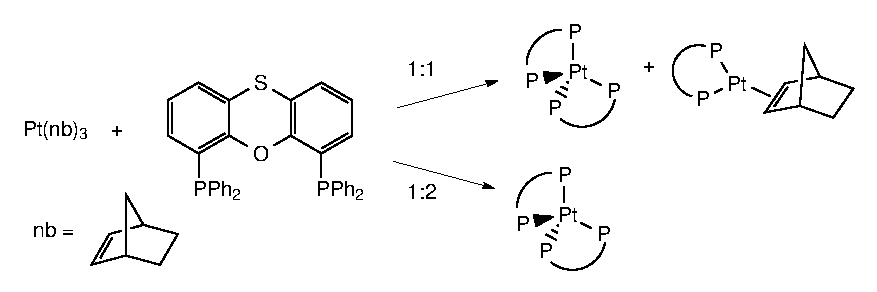
\includegraphics{../Schemes/thixantphosPtnb3.eps}
\caption[Reaction of thixantphos with  tris-(norbornene)platinum]{Reaction of thixantphos with  tris-(norbornene)platinum.}
\label{scheme:PtSPh2}
\end{center}
\end{scheme}

Yellow crystals of [Pt(\Phthixantphos\ce{)2]}$\cdot$2.5 \ce{CH2Cl2} were grown by inwards diffusion of diethyl ether into a dichloromethane solution of the complex.  The complex crystallised in the monoclinic space group C2/c with a well-defined main structure, though some disorder is present in the dichloromethane solvate.  The crystal structure is shown in Figure \ref{crystalbisthixantphosplatinum}, with Figure \ref{crystalbisthixantphosplatinumphenyl} showing the same structure without the phenyl substituents on the phosphorus atoms.  Selected bond lengths and angles are given in Table \ref{table:crystalbisthixantphosplatinum:lengths}, and crystallographic information is given in Table \ref{table:crystalbisthixantphosplatinum:data}.  

%\fixme{bis-thixantphosplatinum} suitable for X-ray crystallography were grown by inwards diffusion of diethyl ether into a dichloromethane solution of [Pt(\Phthixantphos\ce{)2].  The complex crystallised as .  The X-ray crystal structure (Figure \ref{Crystal:bisthixantphosplatinum}) is in the monoclinic space group C2/c.  Selected bond lengths and angles are given in Table \ref{table:crystalbisthixantphosplatinum:lengths} and crystallographic data is given in Table \ref{table:crystalbisthixantphosplatinum:data}. 

\begin{figure}[htbp]
\begin{center}
\vspace{0.5cm}
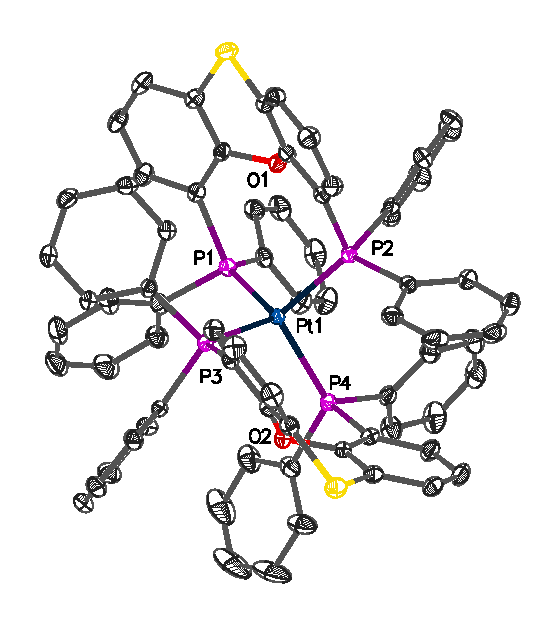
\includegraphics[scale=0.9]{../Figures/CrystalPtSPh2.eps}
\caption[X-ray crystal structure of \ce{[Pt(Ph-thixantphos)2]}]{X-ray crystal structure of \ce{[Pt(Ph-thixantphos)2]}, hydrogen atoms and dichloromethane of crystallisation omitted for clarity}
\vspace{0.2cm}
\label{crystalbisthixantphosplatinum}
\end{center}
\end{figure}
\vspace{0.2cm}

\begin{figure}[htbp]
\begin{center}
\vspace{0.5cm}
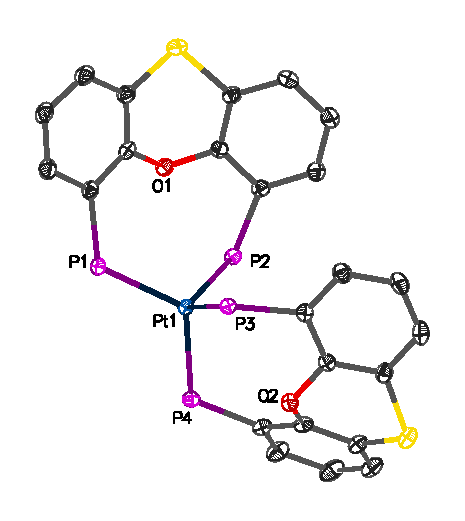
\includegraphics[scale=0.97]{../Figures/CrystalPtSPh2phenyl.eps}
\caption[X-ray crystal structure of \ce{[Pt(Ph-thixantphos)2]}]{X-ray crystal structure of \ce{[Pt(Ph-thixantphos)2]}, hydrogen atoms, dichloromethane of crystallisation and phenyl rings omitted for clarity}
\vspace{0.2cm}
\label{crystalbisthixantphosplatinumphenyl}
\end{center}
\end{figure}
\vspace{0.2cm}

\begin{table}[htp]
\caption[Selected bond distances (\AA) and angles (\degrees) of \ce{[Pt(Ph-thixantphos)2]}]{Selected bond distances (\AA) and angles (\degrees) of \ce{[Pt(Ph-thixantphos)2]}}
\vspace{1em}
\label{table:crystalbisthixantphosplatinum:lengths}
\small
\begin{center}
\begin{tabular}{l l l l}
	\toprule
	\multicolumn{2}{l}{\bfseries{~Bond distances (\si{\angstrom})}} & \multicolumn{2}{c}{\bfseries{Bond angles (\degrees)}} \\
	\midrule		
	~P1-Pt1		~~&~~2.3325(6)~~	&~~P1-Pt1-P2		~~	&~~108.059(17)	\\
	~P2-Pt1		~~&~~2.3209(5)~~	&~~P1-Pt1-P3		~~	&~~105.501(17)	\\
	~P3-Pt1		~~&~~2.3242(4)~~	&~~P1-Pt1-P4		~~	&~~119.313(17)	\\
	~P4-Pt1		~~&~~2.3249(5)~~	&~~P2-Pt1-P3		~~	&~~114.224(19)	\\
	~P1...P2		~~&~~3.7661(7)~~	&~~P2-Pt1-P4		~~	&~~103.741(18)	\\
	~P1...P3		~~&~~3.7068(7)~~	&~~P3-Pt1-P4		~~	&~~106.377(16)	\\
	~P1...P4		~~&~~4.0194(7)~~	&~~Ring 1-Ring 2	~~	&~~35.57(8)		\\
	~P2...P3		~~&~~3.9007(7)~~	&~~Ring 3-Ring 4	~~	&~~45.39(8)		\\
	~P2...P4		~~&~~3.6544(7)~~	&~~				~~	&~~				\\
	~P3...P4		~~&~~3.7221(6)~~	&~~				~~	&~~				\\
	~Pt1...O1		~~&~~3.4977(14)~~	&~~				~~	&~~				\\
	~Pt1...O2		~~&~~3.5635(14)~~	&~~				~~	&~~				\\
	\bottomrule{}
\end{tabular}
\end{center}
\end{table}

\begin{table}[htp]
\small
\caption[Crystallographic Data and Structure Refinement of \ce{[Pt(Ph-thixantphos)2]}]{Crystallographic Data and Structure Refinement of \ce{[Pt(Ph-thixantphos)2]}} 
\vspace{1em}
\label{table:crystalbisthixantphosplatinum:data}
\small
\begin{center}
\begin{tabular}{l l}
	\toprule
	\bfseries{Empirical formula}~~& \bfseries{\ce{C149H114Cl10O4P8Pt2S4}}\\
	\midrule
	Formula weight	 							& 3089.07\\
	Temperature/K	 							& 296.0\\
	Crystal system	 							& monoclinic\\
	Space group	 							& C2/c\\
	a$/$\si{\angstrom}							& 46.8743(16))\\
	b$/$\si{\angstrom} 							& 13.1000(4)\\
	c$/$\si{\angstrom}							& 21.7852(7)\\
	$\alpha/$\degrees							& 90\\
	$\beta/$\degrees							& 105.208\\
	$\gamma/$\degrees							& 90\\
	Volume$/$\si{\angstrom\cubed}  				& 12908.8(7)\\
	Z	 									& 4\\
$\rho$\sub{calc} \si{\milli\gram}$/$\si{\milli\metre\cubed} 	& 1.589\\
\si{\metre}$/$\si{\milli\metre} 						& 2.594\\
F(000)	 									& 6200.0\\
Crystal size$/$\si{\milli\metre\cubed}	 				& 0.61 x 0.18 x 0.15\\
Radiation	 									& MoK$\alpha$ ($\lambda$ = 0.71073)\\
2$\theta$ range for data collection					& 3.602 to 60.916\degrees\\
Index ranges	 								& -66 $\leq$ h $\leq$ 66, -18 $\leq$ k $\leq$ 17, -30 $\leq$ l $\leq$ 30\\
Reflections collected	 							& 172570\\
Independent reflections	 						& 19386 [R\sub{int} = 0.0370, R\sub{sigma} = 0.0207]\\
Data$/$restraints$/$parameters					& 19386$/$0$/$808\\
Goodness-of-fit on F$^{2}$	 					& 1.232\\
Final R indexes [I$>$=2$\sigma$ (I)]	 				& R\sub{1} = 0.0219, wR\sub{2} = 0.0565\\
Final R indexes [all data]	 						& R\sub{1} = 0.0338, wR\sub{2} = 0.0716\\
Largest diff. peak/hole / e \si{\per\angstrom\cubed}		& 1.08/-1.07	\\
	\bottomrule
\end{tabular}
\end{center}
\end{table}

The X-ray crystal structure of [Pt(\Phthixantphos\ce{)2}] shows a distorted tetrahedral configuration with angles ranging from 103.741(18) to 119.313(17)\degrees.  This is likely due to the restrictions caused by having two rigid xantphos ligands around a single metal centre.  There are two different phosphorus environments present in the crystal structure, such that each ligand has each of the two environments.  One phosphine on each ligand is nearer to the adjacent ligand backbone whilst the other phosphine is nearer to the adjacent phenyl substituents.  The backbone is bent away from planarity to allow the ligand to coordinate with bite angles of 106.377(16) and 108.059(17)\degrees. These angles are relatively close to the natural bite angle calculated for this ligand of 109.4\degrees{} from molecular mechanics and are slightly smaller than the DFT calculated value of 118.0\degrees.\cite{Birkholz2009}

Tetrahedral complexes of platinum with four phosphorus donors are well-known with numerous crystallographically determined structures.  One such structure with a xantphos ligand derivatised with ethyl groups on the phosphorus atoms was reported in 2004 (Figure \ref{Etxantphos}).\cite{Miedaner2004}  The [Pt(Et-xantphos\ce{)2}] complex shows a very similar structure to the [Pt(\Phthixantphos\ce{)2}].  The bite-angles for the ethyl complex are 108.07(7) and 108.44(7)\degrees, which are very similar to the \Phthixantphos{} complex of 108.059(17) and 105.501(17)\degrees.  The bite-angle is also very similar to a [Pd(\Phxantphos\ce{)2}] complex which has P-Pd-P angles of 106.33\degrees. \fixme{esd, cite grushin2006} Given these similarities it is likely that the geometry of the complexes and the bite-angles of the ligand in these complexes are controlled mostly by valence angles.  \fixme{possibly rethink this sentence - John}

\begin{figure}[htb]
\begin{center}
\vspace{0.5cm}
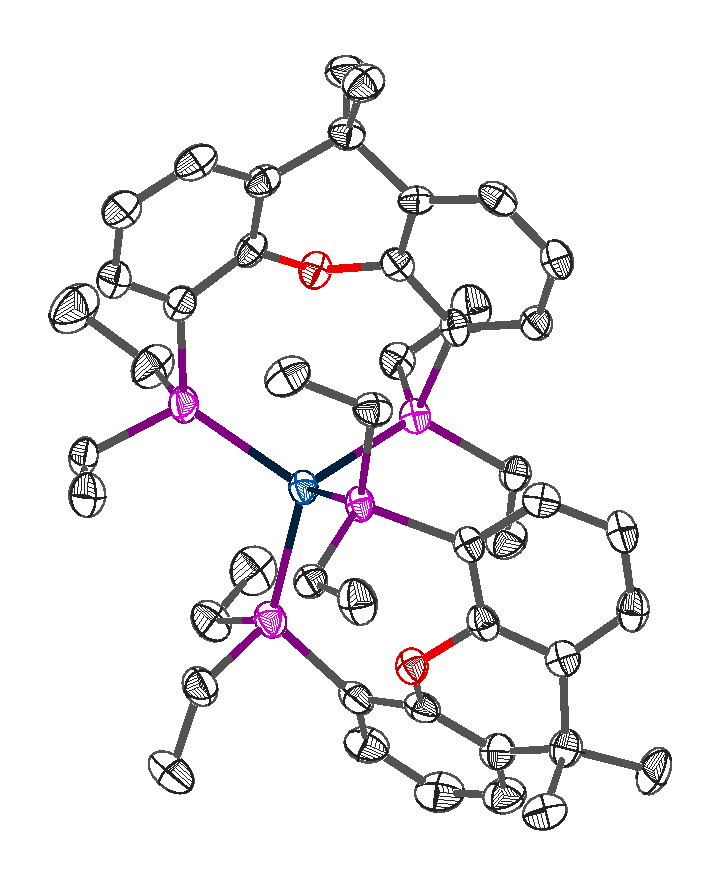
\includegraphics[scale=0.7]{../Othercrystals/Etxantphos.eps}
\caption[X-ray crystal structure reported for [Pt(Et-xantphos\ce{)2}{]}]{X-ray crystal structure reported for [Pt(Et-xantphos\ce{)2}].  Hydrogen atoms omitted for clarity.\cite{Miedaner2004}}
\vspace{0.2cm}
\label{Etxantphos}
\end{center}
\end{figure}
\vspace{0.2cm}

The X-ray crystal structure of [Pt(\Phthixantphos\ce{)2}] shows two different phosphorus environments, for each \Phthixantphos{} ligand (Figure \ref{crystalbisthixantphosplatinumphenyl}).  The backbone of the \Phthixantphos{} ligand is curved in the crystal structure.  One of the phosphorus atoms on one of the ligands sits within the concave face of the  other ligand's backbone while the convex face of this backbone points away from the centre of the complex.  The other phosphorus atom from the same ligand sits below the ligand and has closer contacts with the phenyl substituents than the backbone.  This indicates that while the two ligands are related overall, the two halves of a single ligand are in quite different spacial environments.  

From the X-ray crystal structure of [Pt(\Phthixantphos\ce{)2}] we would expect the \phosphorus{} NMR spectrum to show two different phosphorus environments.  At room temperature both the \proton{} and \phosphorus{} NMR spectra are very broad.  While two environments are present in the \phosphorus{} NMR spectrum, no coupling can be readily discerned.  This suggests that a dynamic process occurs, which was further investigated by variable temperature NMR analysis in \ce{CD2Cl2}.  Upon lowering the temperature to 0 \degC, the \phosphorus{} NMR spectrum (Figure \ref{BisSPhPt:PNMR}) has become much sharper and coupling can be observed on the main peaks and platinum satellites are also apparent.  This system continues to sharpen down to around -40 \degC, below which no further changes are observed.  The low temperature \proton{} NMR spectra (Figure \ref{BisSPhPt:HNMR}) show a similar pattern.  The system shows dramatic sharpening upon cooling to 0 \degC, which continues down to -40 \degC.  However, unlike the \phosphorus{} NMR, the \proton{} NMR spectra at -60 and -80 \degC{} begin to broaden once more.

As mentioned when discussing the [Ag(\tButhixantphos)Cl] complex (Chapter \ref{ch:silver}) the xantphos backbones frequently bend in order to achieve the coordination angles desired by the metal.  However, while this is seen in the crystal structures of the complexes it is not observed in the NMR spectra due to rapid inversion of the ligand such that both faces of the backbone are the same, on the NMR timescale.  In the case of [Pt(\Phthixantphos\ce{)2}] the X-ray crystal structure shows the two different spatial phosphorus environments which should result in different chemical shifts in the \phosphorus{} NMR spectrum.  This system is sufficiently crowded around the metal centre to reduce the ability of the xantphos system to invert.  As such cooling to 0 \degC{} is sufficient to lock the backbones of [Pt(\Phthixantphos\ce{)2}] in a single configuration.  Thus allowing the two different \phosphorus{} environments to become visible.  Even at room temperature two different signals are apparent, indicating that although the inversion is occurring the rate is slow enough compared to the NMR timescale to allow some distinction between the two phosphorus atoms.  The inversion of the xantphos backbones stops upon cooling to around -20 \degC.  However, while the \phosphorus{} NMR spectrum remains sharp below this temperature the \proton{} spectrum begins to broaden again.  This may be the result of restricted rotation of some or all of the phenyl rings which may occur due to the steric demands of the system.  

\begin{figure}[htbp]
\begin{center}
\vspace{0.5cm}
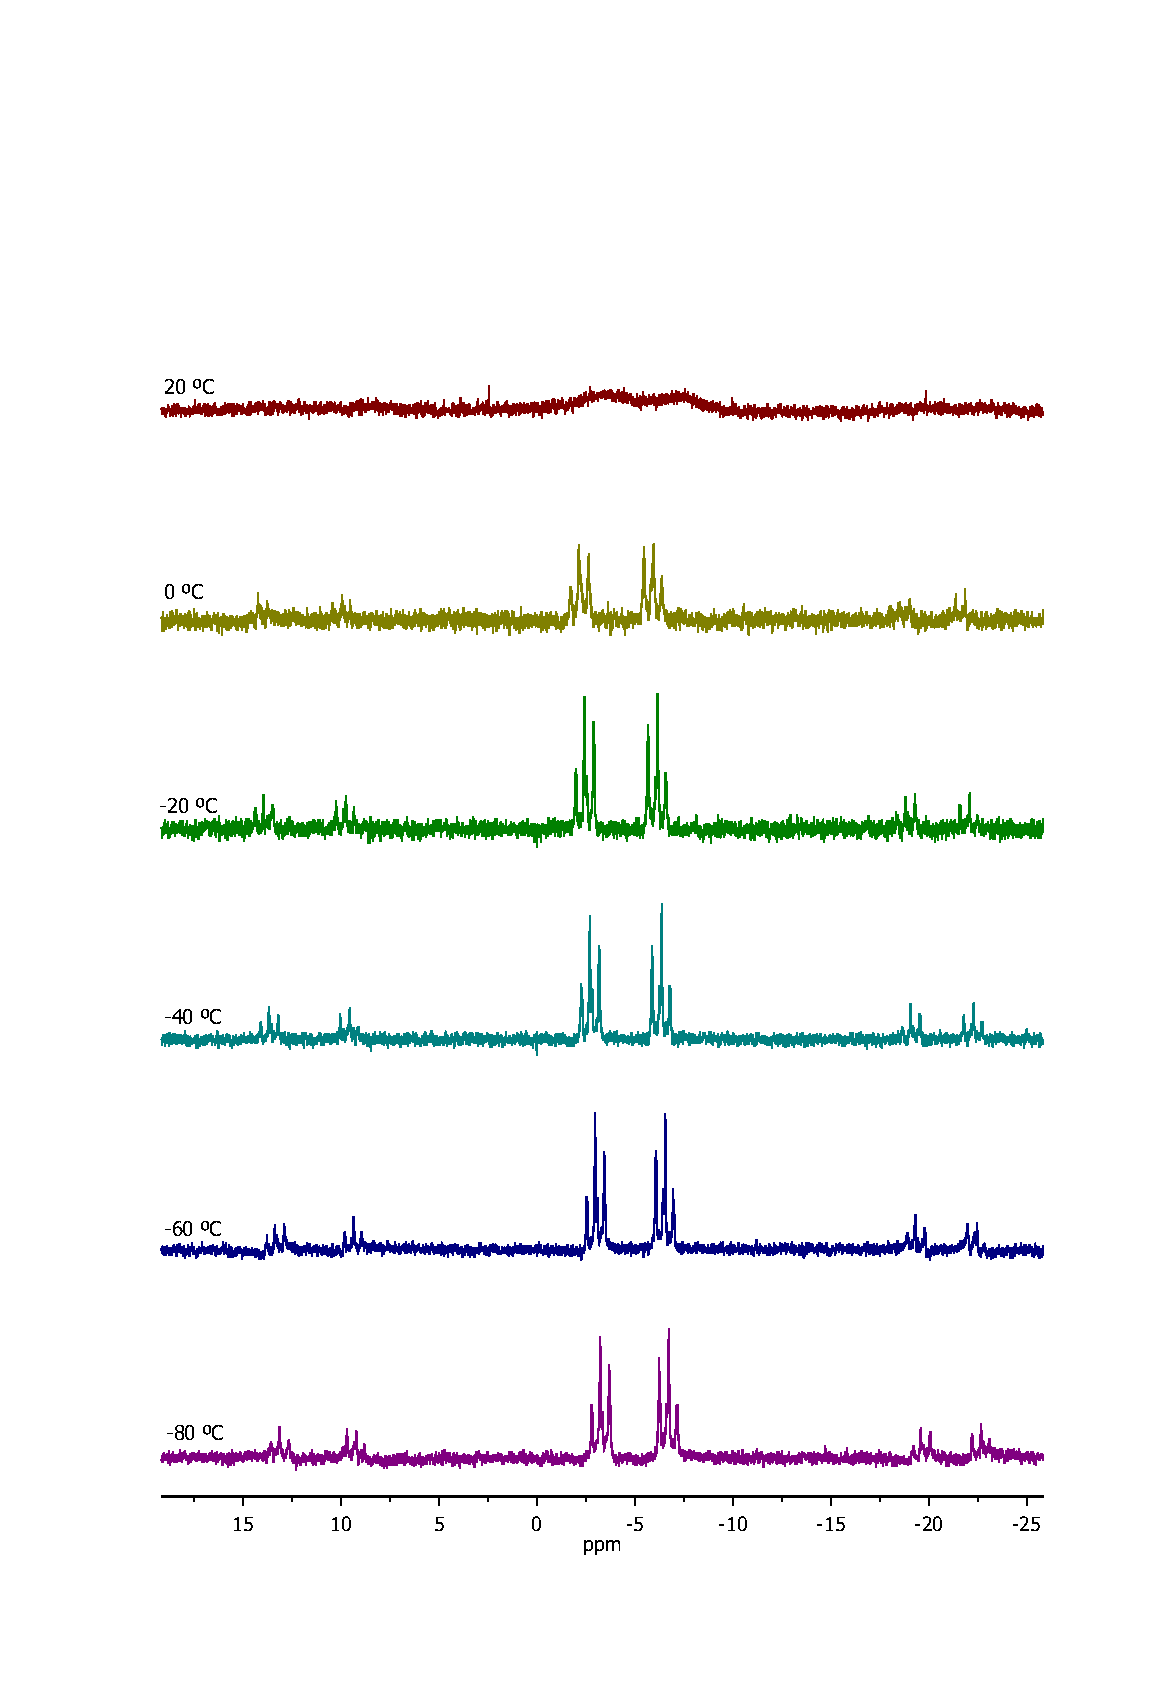
\includegraphics[scale = 0.9, trim = 2cm 1.5cm 1.5cm 4cm, clip]{../NMR/1031-Pt(SPh)2-2.eps}
\caption[Low temperature \phosphorus{} NMR spectra for [Pt(Ph-thixantphos\ce{)2}{]}]{Low temperature \phosphorus{} NMR spectra for [Pt(Ph-thixantphos\ce{)2]} in \ce{CD2Cl2}}
\vspace{0.2cm}
\label{BisSPhPt:PNMR}
\end{center}
\end{figure}
\vspace{0.2cm}

\begin{figure}[htbp]
\begin{center}
\vspace{0.5cm}
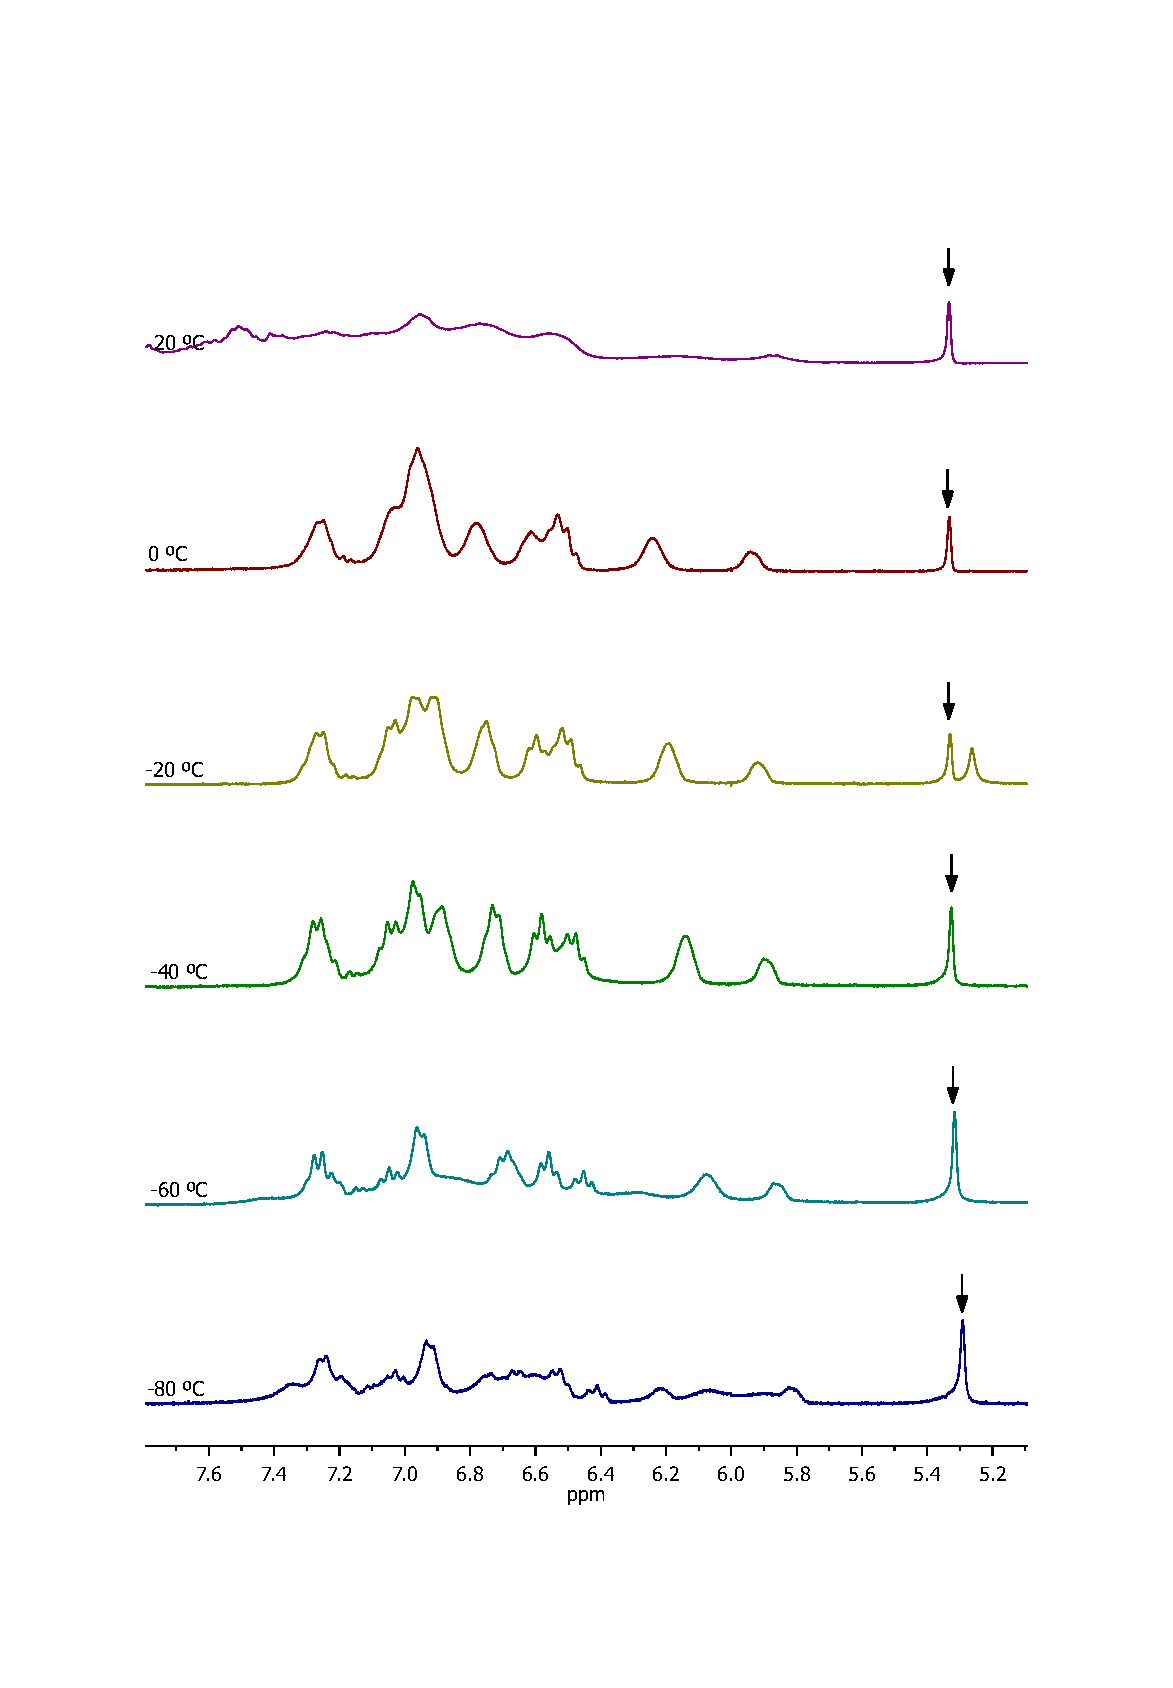
\includegraphics[scale = 0.9, trim = 2cm 2.5cm 1.7cm 4cm, clip]{../NMR/1031-Pt(SPh)2-Proton.eps}
\caption[Low temperature \proton{} NMR spectra for [Pt(Ph-thixantphos\ce{)2}{]}]{Low temperature \proton{} NMR spectra for [Pt(Ph-thixantphos\ce{)2]}, showing the aromatic region.  The solvent \ce{CD2Cl2} is indicated by an arrow.}
\vspace{0.2cm}
\label{BisSPhPt:HNMR}
\end{center}
\end{figure}
\vspace{0.2cm}

The \phosphorus{} NMR spectrum of [Pt(\Phthixantphos\ce{)2}] at -80 \degC{} shows some interesting features.  Two peaks are observable as triplets at -2.43 and -6.16 ppm with phosphorus-phosphorus coupling of 55.0 Hz and platinum satellites of 3976 and 3864 Hz respectively.  The value for the phosphorus-phosphorus coupling is slightly larger than that reported for the analogous [Pt(Et-xantphos\ce{)2}] complex which showed two triplets at -6.82 and -19.65 ppm with two-bond, phosphorus-phosphorus coupling of 48 Hz.\cite{Miedanar2004}  The phosphorus-platinum coupling constants were also very similar between the two complexes.  The \Phthixantphos{} complex had coupling constants of 3976 and 3864 Hz while the Et-xantphos complex showed 4086 and 3602 Hz.  This indicates a remarkable similarity between the two complexes, again indicating that the geometry of the system is controlled mostly by the metal centre.  However, the \phosphorus{} NMR spectrum of [Pt(Et-xantphos\ce{)2}] was sharp at room temperature in toluene-\ce{d8} indicating that the propensity for these complexes to undergo inversion differs.\cite{Miedanar2004}

A useful platinum(0) starting materials is tris-(ethene)platinum.  The ethene ligands are readily displaced by other ligands, though [Pt(\ce{C2H4)3}] is only stable under an ethene atmosphere. Transition metal ethene complexes are very important from an industrial perspective as ethene is one of the most common feedstocks used in the petrochemical industry.  Reaction between [Pt(\ce{C2H4)3}] and \Phthixantphos{} was carried out on an NMR scale to allow the identification of any intermediates that may form.  The reaction was very quick and the solution turned orange after only 10 mins at room temperature.  By \phosphorus{} NMR [Pt(\Phthixantphos\ce{)2}] was the major product accounting for 93\% of the phosphorus containing species while the remaining 7\% is [Pt\ce{(C2H4)}(\Phthixantphos)] (Scheme \ref{scheme:PtSPhEt}) analogous to the [Pt(nb)(\Phthixantphos)] formed in reaction with [Pt(nb\ce{)3]}.  Interestingly the ratio of the alkene to bis complex appears to be dependent on the alkene used.  The small amount of [Pt\ce{(C2H4)}(\Phthixantphos)] formed suggests that the free ligand prefers to react with the alkene complex to form [Pt(\Phthixantphos\ce{)2]} rather than react with [Pt\ce{(C2H4)3}].  Thus suggesting that the initial coordination of the diphosphine to form [Pt\ce{(C2H4})(\Phthixantphos)] activates the system to react further with free \Phthixantphos.  However, in the norbornene case we observe 60.4\% [Pt(\Phthixantphos\ce{)2}] indicating that while the uncoordinated diphosphine does prefer to react with [Pt(nb)(\Phthixantphos)] over the [Pt(nb\ce{)3}], the effect is not as significant as for the ethene system.  

\begin{scheme}[ht]
\begin{center}
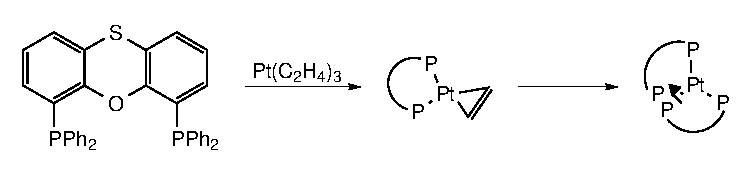
\includegraphics{../Schemes/thixantphosPtEt.eps}
\caption[Reaction of thixantphos with  tris-(ethene)platinum]{Reaction of thixantphos with  tris-(ethene)platinum}
\label{scheme:PtSPhEt}
\end{center}
\end{scheme}

\section{Reaction of \tBuxantphos{} ligands with tris-(norbornene)platinum}  

The equimolar reaction of tris-(norbornene)platinum with \Phthixantphos{} resulted in [Pt(\Phthixantphos\ce{)2}] and [Pt(nb)(\Phthixantphos)] as the major and minor products respectively.  The same reaction was performed using \tButhixantphos{} which differs from \Phthixantphos{} both in the replacement of the phenyl substituents on the phosphorus atoms with \tBu{} groups and the presence of methyl substituents on the backbone positions \emph{meta} to the phosphorus atoms.  Reaction of \tButhixantphos{} with [Pt(nb\ce{)3}] in \ce{C6D6} was slower, requiring heating at 60\degC{} for 4 days in order to go to completion.  Like the reaction with \Phthixantphos{}, the \tButhixantphos{} reaction with tris-(norbornene)platinum also produces two products.  One of these products is the same in both cases, [Pt(diphosphine)(nb)] (diphosphine = \Phthixantphos, \tButhixantphos).  However, rather than a bis-diphosphine complex forming, as observed with \Phthixantphos{}, using \tButhixantphos{} generated a reactive, 14-electron [Pt(\tButhixantphos)] complex (Scheme \ref{scheme:StBuPtnb}).  \fixme{relative ratios?}  Although 14-electron complexes are electron deficient, several examples have been reported with \ce{[Pt(PPh3)2]} first reported in 1966\cite{Ugo1966} followed by \ce{[Pt(PCy3)2]} in 1975\cite{Green1975b} and \ce{[Pt(P^{t}Bu3)2]}, \ce{[Pt(P^{t}Bu2Ph)2]} and \ce{[Pt(P^{i}Pr3)2]} in 1976.

%When the reaction between tris-(norbornene)platinum was carried out with the tertiary butyl substituted thixantphos a different result was observed.  Similarly to the reaction with the phenyl derivative an initial mixture of products was obtained.  In this case both are 1:1 complexes tBu-thixantphos:platinum.  Like the phenyl derivative one of the products is platinum thixantphos norbornene.  The other product is the two-coordinate 14-electron complex platinum thixantphos (Scheme \ref{scheme:StBuPtnb}).  \fixme{give references to these things}  

%The platinum norbornene complex exists only in the presence of excess norbornene and can readily be converted to the 14-electron complex by removing the norbornene \emph{in vacuo}.  

\begin{scheme}[h]
\begin{center}
\vspace{0.5cm}
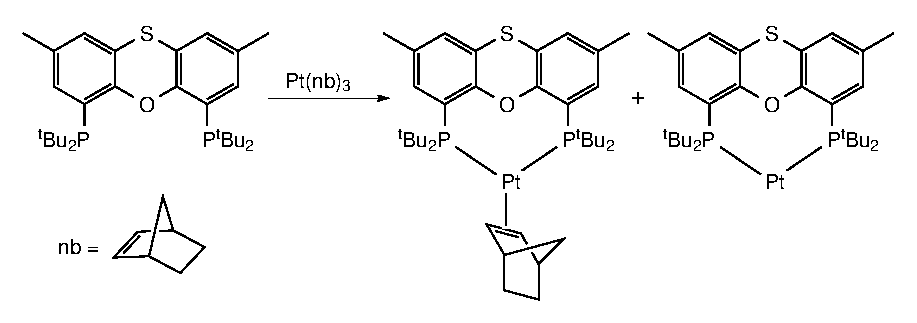
\includegraphics{../Schemes/StBuPtnb.eps}
\caption[Reaction between tBu-thixantphos and tris-(norbornene)platinum]{Reaction between tBu-thixantphos and tris-(norbornene)platinum.}
\vspace{0.2cm}
\label{scheme:StBuPtnb}
\end{center}
\end{scheme}
\vspace{0.2cm}

%\fixme{Why is there a random black spot between my scheme and my caption?}

The [Pt(nb)(\tButhixantphos)] complex exhibits a broad resonance at 55.6 ppm in the \phosphorus{} NMR spectrum with platinum satellites of 3612 Hz.  This \JPtP{} coupling constant is typical for tridentate platinum alkene complexes.  The alkene protons appear at 2.37 ppm as a broad singlet with no discernable phosphorus coupling but platinum coupling of 67.8 Hz, and a similarly broad singlet in the \carbon{} NMR spectrum at 51.9 ppm with \JPtC{} = 343.9 Hz.  Half of the expected number of norbornene and \tButhixantphos{} NMR signals are observed indicating a symmetrical complex.

The reaction between \tBusixantphos{} and \ce{[Pt(nb)3]} was performed under the same conditions.  This reaction shows the formation of an analogous 14-electron [Pt(\tBusixantphos)] complex appearing at 79.5 ppm (\JPtP{} = 4827 Hz) as the major product after 24 hours at 60 \degC.  Two other products are also observed, appearing at 59.3 ppm (\JPtP{} = 3572 Hz) and 34.7 ppm (\JPtP{} = 2677 Hz).  The complex at 59.3 ppm is similar in both chemical shift and coupling constant to [Pt(nb)(\tButhixantphos)], it can be proposed as [Pt(nb)(\tBusixantphos)].  The nature of the complex at 34.7 ppm is unexpected.  The value of \JPtP{} is similar to a number of Pt(II) complexes with \trans{} phosphorus atoms (for examples see Chapter \ref{ch:platinumII}).  Unfortunately the complexes could not be separated to gain further insight into their structures.

\tBuXantphos{} also reacted differently with \ce{[Pt(nb)3]} compared to the other xantphos ligands.  A small amount of a complex at 78.9 ppm, consistent with a [Pt(\tBuxantphos)] complex (the peak in the \phosphorus{} NMR spectrum was too weak to observe any platinum coupling).  However, the major product, and the only species present after 24 hours at 60\degC{} was a complex at 46.7 ppm (\JPtP{} = 3246 Hz).  The \proton{} NMR spectrum of this complex showed a triplet at -18.49 ppm, with equal coupling the phosphorus atoms of 13.1 Hz and platinum of 1107 Hz.  The chemical shift of this signal and the value of \JPtH{} are consistent with a hydride positioned \trans{} to a ligand with a low \trans{}-influence.  The value of \JPH{} is consistent with a \cis{} arrangement of the hydride with the two phosphorus atoms.  The \proton{} and \carbon{} NMR signals for the \tBu{} substituents are broad which may suggest a dynamic process occurring.  The \emph{O}-ipso carbon shows a downfield shift of 2.8 ppm which is consistent with coordination of the oxygen atom.  This leads us to propose a platinum(II) complex of the type [Pt(\tBuxantphosk)H]X.  However, complexes of this type typically have platinum-phosphorus coupling constants of between 2300 and 2800 Hz, while \JPtP{} for this complex is higher at 3246 Hz.  The nature of the counterion, and the hydride source were not determined.  

The formation of [Pt(\tBuxantphosk)H]X likely results from the 14-electron complex undergoing reaction with a component of the system.  Despite the number of \ce{[Pt(monophosphine)2]} complexes, isolatable [Pt(diphosphine)] complexes are relatively rare as the diphosphines typically provide less protection of the metal centre due to the restrictions of their bite-angle.  This means that although [Pt(diphosphine)] complexes are frequently proposed as intermediates, few have been isolated.\cite{Clark1986b, Hackett1988, Nicolas2012}.  The [Pt(diphosphine)] complexes will typically coordinate to any possible ligand that is present.  For example, the proposed 14-electron complex [bis(dicyclohexylphosphino)ethane]platinum, which is formed from the reductive elimination of neopentane from the corresponding hydridoneopentyl complex, reacts with alkenes and alkynes to form [Pt(alkene)(dcype)] or [Pt(alkyne)(dcype)], and reacts with alkanes to form [Pt(alkyl)(dcype)H] complexes.  The diphosphine intermediate also reacts with benzene to form [Pt\ce{(C6H5)(dcype)H]}.  Although in the [Pt(\tBuxantphosk)H]X system no evidence of a coordinated alkyl, phenyl or other fragment was observed, this may explain the formation of the hydride species which may then lose the other ligand to form a counterion.  

The [Pt(\tButhixantphos)] complex can be isolated by removal of the norbornene from the sample, under reduced pressure, while the analogous \tBusixantphos{} and \tBuxantphos{} complexes were too short-lived to be isolated.  The \phosphorus{} NMR data for the complexes is given in Table \ref{table:Pt14NMR}.  The complexes all exhibit single peaks in the \phosphorus{} NMR spectrum shifted downfield from the free ligand by 68 - 71 ppm.  A study of the \phosphorus{} NMR properties of [Pt\ce{(PR3)2}] complexes showed that all the 14-electron complexes of this type that were studied display a downfield shift of the phosphorus signal by between 48 and 58 ppm upon coordination, with platinum-phosphorus coupling constants between 4100 and 4600 Hz.\cite{Mann1980}  The change in chemical shift for the \tBuxantphos{} complexes is larger than that reported for monophosphines.  This may be the result of strain placed on the system to achieve such a larger bite-angle, or the result of a slightly bent complex which may form due to the restrictions on the bite-angles of these ligands.  The platinum-phosphorus coupling is also larger than those previously reported by over 200 Hz.  The largest previously reported Pt-P coupling for these complexes is 4592 for [Pt(\ce{P^{t}Bu2Ph})2], and coupling constants of between 4370 and 4424 have been reported by our group for complexes \fixme{Kathryn's PS, PS=O and PN}.  \fixme{cite Kathryn's thesis}.  The larger coupling constants for the \tBuxantphos{} species likely indicates a distortion of the system from the linearity observed with monophosphine systems.  

\begin{table}[htbp]
\caption[\phosphorus{} NMR data for [Pt(\tBuxantphos){]} complexes]{\phosphorus{} NMR data for [Pt(\tBuxantphos){]} complexes}
\vspace{1em}
\label{table:Pt14NMR}
\small
\begin{center}
\begin{tabular}{l c c c}
\toprule{}
	~~ & \multicolumn{3}{c}{\bfseries{\phosphorus}} \\
	\cmidrule(lr){2-4}
	\bfseries{Diphosphine}&\bfseries{$\delta/$ppm}&\bfseries{$\Delta\delta/$ppm}&\bfseries{\JPtP}\\
	\midrule{}
	\tBuSixantphos 		& 79.5 & 71.1 & 4827 \\
	\tBuThixantphos 	& 78.6 & 69.1 & 4810 \\
	\tBuXantphos		& 78.9 & 68.7 & n.o.\\
	\bottomrule{}
\end{tabular}
\end{center}
\end{table}

\section{Reaction of \tButhixantphos{} with \texorpdfstring{\ce{Pt(COD)2}} P}

Bis-(1,5-cyclooctadiene)platinum readily loses \gls{cod} and is commonly used starting material for the formation of platinum(0) phosphine complexes.  The reaction between \tButhixantphos{} and [Pt(COD\ce{)2}] was carried out on an NMR scale in \ce{C6D6}.  The only phosphorus containing product of the reaction is [Pt(\tButhixantphos)].  However, conversion of only 28\% was achieved.  After 48 hours at room temperature the reaction had become black and despite heating no further reaction was observed.  Together with the absence of unreacted [Pt(COD\ce{)2}] in the \proton{} NMR spectrum suggests that the [Pt(COD\ce{)2}] was unstable under the reaction conditions.  Analysis of the reaction by \proton{} and \carbon{} NMR showed the presence of 1,3- and 1,4-cyclooctadiene in addition to 1,5-cyclooctadiene.  Furthermore a very small signal in the \proton{} NMR spectrum appeared at -18.2 ppm as a triplet (\JPH{} = 13.7 Hz) with platinum satellites (\JPtH{} = 1100 Hz).  This signal is in a similar position and has similar coupling constants to the peak in the \proton{} NMR of [Pt(\tBuxantphos)H]X.  This may indicate that the 14-electron [Pt(\tButhixantphos)] complex is able to catalyse the isomerisation of the 1,5-cyclooctadiene.  This process may involve the oxidative addition of an allylic C-H of the COD ligand, to the platinum forming an \hapto{3}-allyl which could then reductively eliminate to form the 1,3-cyclooctadiene.  \fixme{I should put a scheme here}  Given the poor reactivity of [Pt(COD\ce{)2}] with \tButhixantphos{} the analogous reactions with \tBusixantphos{} and \tBuxantphos{} were not attempted.  \fixme{think through this as John think I'm missing a step.  John thinks I need to draw a scheme and then describe the scheme}

%A reaction between \emph{bis}-1,5-cyclooctadiene platinum and tBu-thixantphos resulted in exclusively the 14-electron complex.  However, upon completion of the reaction peaks were observed in the \proton{} and \carbon{} NMR spectra corresponding to 1,3- and 1,4-cyclooctadiene as well as 1,5-cyclooctadiene, this was further confirmed by gas chromatography mass spectrometry analysis of the sample.\fixme{get relative ratios?}  An intermediate was observed with a high field triplet in the \proton{} NMR at -18.2 ppm (\JPH{} = 13.7, \JPtH = 1100).  This indicates that the cyclooctadiene was likely undergoing a C-H activation reaction followed by isomerisation of the double bonds and then reductive elimination to give the different isomers.  

\section{Reaction of \tBuxantphos{} ligands with \texorpdfstring{\ce{[Pt(C2H4)3}]} P}

Ethene is an important feedstock for industrial processes, which can include transition metal ethene complexes as intermediates.  Ethene is a smaller alkene than both 1,5-cyclooctadiene and norbornene we may see different reactivity due to the lower steric restrictions upon forming alkene complexes.  The three \tBuxantphos{} ligands were reacted on an NMR-scale in \ce{C6D6}, with freshly prepared [Pt\ce{(C2H4)3}] made from [Pt(COD\ce{)2}] under an ethene atmosphere.  All three ligands firstly formed a complex of the type [Pt(\tBuxantphos{})(\ce{C2H4})].  However, while the ethene complex was the only product for \tButhixantphos, the reaction with \tBuxantphos{} progressed to form [Pt(\tBuxantphos)H]X.  Again the nature of the counterion in this species was unable to be determined.  \fixme{talk about what happens with \tBusixantphos{}}

Selected NMR data for these complexes is outline in Table \ref{table:PtEtNMR}.  In all cases the \phosphorus{} NMR spectrum shows a singlet at between 53.4 and 55.7 ppm shifted downfield by between 43.2 and 46.2 ppm from the corresponding free ligand.  [Pt(\tBusixantphos{})(\ce{C2H4})] has a \JPtP{} value almost 400 Hz lower than that observed for the corresponding \tButhixantphos{} and \tBuxantphos{} complexes.  All are within the expected range for complexes of this type \fixme{reference the NMR book}.  The lower coupling constant may indicate that the ethene ligand is more strongly coordinated to the platinum centre.  This may be the result of the smaller bite-angle of the \tBusixantphos{} ligand allowing more room for the ethene ligand to interact with the platinum.  The \proton{} NMR spectrum showed peaks at 2.50 and 2.52 corresponding to the ethene protons for the [Pt(\tButhixantphos{})(\ce{C2H4})] and [Pt(\tBuxantphos{})(\ce{C2H4})] respectively.  The dramatic upfield shift of the ethene ligand is consistent with coordination to a metal centre such at platinum (uncoordinated ethene appears at 5.25 ppm\cite{Fulmer2010}).  As both the \tBusixantphos{} and \tBuxantphos{} ethene complexes reacted further to produce mixtures, the \carbon{} peak for the ethene ligand was only observed in [Pt(\tButhixantphos{})(\ce{C2H4})].  The ethene carbon appeared at 34.2 ppm as a broad signal with platinum satellites of 223.2 Hz, consistent with this type of complex.  

\begin{table}[htbp]
\caption[\phosphorus{} NMR data for [Pt(\tBuxantphos)(C2H4){]} complexes]{\phosphorus{} NMR data for [Pt(\tBuxantphos)(C2H4{]} complexes}
\vspace{1em}
\label{table:PtEtNMR}
\small
\begin{center}
\begin{tabular}{l c c c c c}
\toprule{}
	~~ & \multicolumn{3}{c}{\bfseries{\phosphorus}} \\
	\cmidrule(lr){2-4} \cmidrule(lr){5-6}
	\bfseries{Diphosphine}&\bfseries{$\delta/$ppm}&\bfseries{$\Delta\delta/$ppm}&\bfseries{\JPtP $/$Hz} & \bfseries{$\delta/$ppm} & \bfseries{\JPtH $/$Hz} \\
	\midrule{}
	\tBuSixantphos 		& 53.7 & 45.3 & 3499 & \fixme{n.o.} & \fixme{n.o.} \\
	\tBuThixantphos 	& 55.7 & 46.2 & 3899 & 2.50 & 59.5 \\
	\tBuXantphos		& 53.4 & 43.2 & 3878 & 2.52 & 58.0 \\
	\bottomrule{}
\end{tabular}
\end{center}
\end{table}

%Ligand \fixme{ref} tBu-Thixantphos was reacted with tris-(ethene)platinum. In order to investigate the role of sterics on the position of the equilibrium between the norbornene complex and the 14-electron complex.  The ligand was added to freshly synthesised tris-(ethene)platinum and reacted under an ethene atmosphere.  A single product was observed in the \phosphorus{} NMR spectrum at 55.7 ppm (\JPtP{} = 3899.1 Hz) which was identified as a tBu-thixantphos platinum ethene complex (Scheme \ref{scheme:StBuPtethene}).  A single signal for the ethene was observed in the \proton{} and \carbon{} NMR spectra at 2.50 ppm (\JPtH{} = 59.5 Hz) and 34.2 ppm (\JPtC{} = 223.2 Hz).  This indicates that either the ethene is freely rotating in solution or the backbone of the ligand is inverting resulting in averaged identical averaged proton environments.  

\begin{scheme}[ht]
\begin{center}
\vspace{0.5cm}
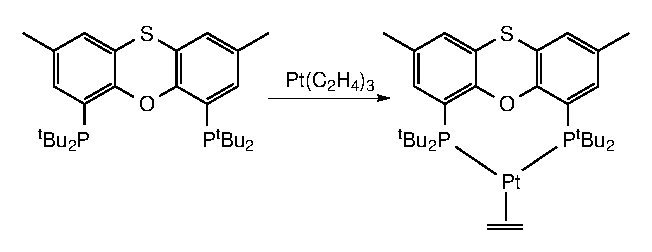
\includegraphics{../Schemes/StBuPtethene.eps}
\caption[Reaction between tBu-thixantphos and tris-(ethene)platinum platinum]{Reaction between tBu-thixantphos and tris-(ethene)platinum platinum.}
\vspace{0.2cm}
\label{scheme:StBuPtethene}
\end{center}
\end{scheme}
\vspace{0.2cm}

The three reactions with the alkenes show markedly different results.  With norbornene an equilibrium forms between [Pt(\tButhixantphos)nb] and [Pt(\tButhixantphos)].  With [Pt(cod\ce{)2}] only [Pt(\tButhixantphos)] forms, and with [Pt\ce{(C2H4)3}] only [Pt(\tButhixantphos)(\ce{C2H4})] results. [Pt(\tButhixantphos)(nb)] was converted entirely to the [Pt(\tButhixantphos)] complex by placing a sample under vacuum for one hour, while the [Pt(\tButhixantphos)\ce{(C2H4)}] complex showed no change under the same conditions.  Bubbling argon through a solution of [Pt(\tButhixantphos)\ce{(C2H4)}] for \fixme{time} resulted in only small amounts of the 14-electron complex forming.  This indicates that the ethene is more strongly coordinated to the platinum than the norbornene and is less prone to dissociation.  Dialkyl substituted alkenes are poorer ligands when compared with ethene, as shown in the straightforward synthesis of [Pt(\ce{C2H4)3}] from [Pt(cod\ce{)2}].  However, coordination of norbornene relieves some of the ring-strain which means it coordinates more strongly than cod.  [Pt(nb\ce{)3}] is an air-stable solid, while [Pt(\ce{C2H4})3] degrades if not stored under ethene.  This suggests that the relief of ring strain may be sufficient to overcome the electronic factors describes by Tolman \fixme{citations?}

%This is contrary to what is expected given that COD is the strongest binding of the three alkenes due to the chelate effect and the NMR data for the ethene and norbornene complexes indicates that the ethene is less strongly bound to the platinum than the norbornene (\JPtC{} = 223.2 and 343.9 Hz respectively).  The presence of a large excess of ethene by working under an ethene atmosphere may be sufficient to push the equilibrium towards the ethene complex, however the reaction in both cases would produce two equivalents of excess alkene so this is unlikely to make a significant difference.  

The predominating factor governing the coordination behaviour of the three alkenes in \tButhixantphos{} platinum complexes is likely to be sterics.  \Gls{cod} is the largest of the three alkenes, followed by norbornene, then ethene \fixme{get cone angles or a reference or something}.  The \tButhixantphos{}ligand has a calculated natural bite-angle of 131\degrees and has large tertiary butyl groups resulting in a large cone angle\fixme{probably best to get some data on this}.  As such the molecule is put under strain by the addition of larger alkenes which offset the additional stability that the alkenes afford in coordinating to the metal centre.  As \gls{cod} is the largest of the three the final complex shows none of the alkene complex whilst the ethene as the smallest is exclusively the ethene complex.  However, norbornene being of an intermediate size forms an equilibrium with both the norbornene complex and the 14-electron complex coexisting.  

 %so there is more strain present in the molecule when the norbornene is bound compared to ethene which counteracts the added stability from having a 16-electron metal centre.  This strain results in a higher energy complex with little barrier to norbornene loss and little energy different between the norbornene complex and the 14-electron complex, thus resulting in an equilibrium.  In the ethene there is very little strain induced from the ethene and the additional electron density on the platinum results in the ethene complex being much lower in energy and thus no equilibrium is present between the ethene and the 14-electron complex.  
 
\section{Formation of platinum dioxygen complexes}

14-electron platinum complexes are commonly reactive towards small molecules, particularly those with diphosphine ligands as was observed with [Pt(\tBusixantphos)] and [Pt(\tBuxantphos)].  \fixme{first sentence needs citations}The reactivity of [Pt(\tButhixantphos)] is lower than the reactivity of the corresponding \tBusixantphos{} and \tBuxantphos{} complexes.  Both the \tBusixantphos{} and \tBuxantphos{} complexes were unstable in solution, while the \tButhixantphos{} complex was stable in \ce{C6D6}, under argon, at room temperature for at least several days.  However, [Pt(\tButhixantphos)] was highly reactive towards oxygen and would readily form [Pt(\tButhixantphos)\hapto{}-\ce{O2}] upon exposure to air (Scheme \ref{scheme:StBuPtO2}).  Bubbling air through a reaction mixture containing [Pt(\tButhixantphos)] and [Pt(\tButhixantphos)(nb)] or a sample of [Pt(\tButhixantphos)(\ce{C2H4})] resulted in complete conversion (by \phosphorus{} NMR spectroscopy) to [Pt(\tButhixantphos)\hapto{}-\ce{O2}].  This reaction is quite common for complexes of the type [Pt(\ce{PR3)2})]\cite{Goel1983b, Yoshida1977}

\begin{scheme}[ht]
\begin{center}
\vspace{0.5cm}
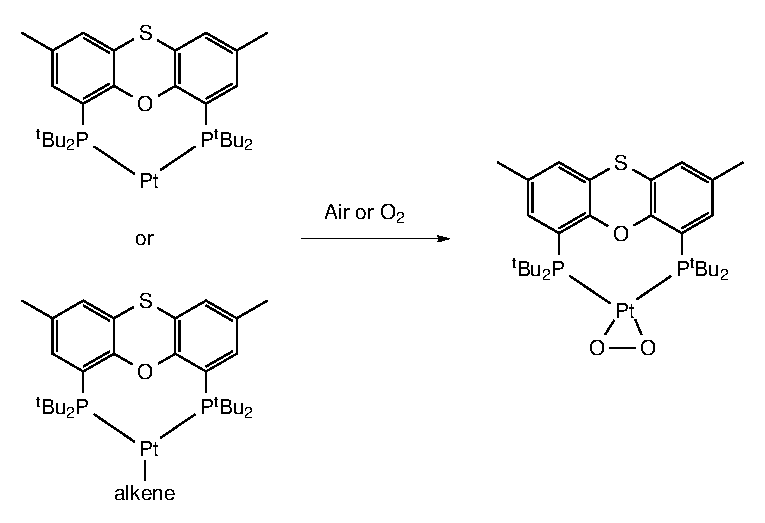
\includegraphics{../Schemes/StBuPtO2.eps}
\caption[Reaction of [Pt(alkene)(\tButhixantphos){]} and [Pt(\tButhixantphos){]} with air]{Reaction of [Pt(alkene)(\tButhixantphos){]} and [Pt(\tButhixantphos){]} with air.  Alkene = \ce{C2H4} or norbornene.}
\vspace{0.2cm}
\label{scheme:StBuPtO2}
\end{center}
\end{scheme}
\vspace{0.2cm}

Upon reaction of [Pt(\tButhixantphos)] with oxygen the \phosphorus{} NMR signal shifts upfield from 78.6 to 38.4 ppm with an associated reduction in the magnitude of the phosphorus-platinum coupling from 4810 to 4488 Hz.  The reduction in coupling constant is a result of the decrease in the s-character of the platinum bond orbitals upon changing the geometry of the complex.\cite{Pregosin2012}  The value of the \JPtP{} coupling constant is larger than those previously reported (3930 - 4112 Hz).\cite{Goel1983b} \fixme{cite Kathryn}.  Similarly to the NMR data obtained for [Pt(\tButhixantphos)] these values may be different from the literature data due to the constraints of the diphosphine ligand over the monophosphines reported in the literature.  The \proton{} and \carbon{} NMR spectra of [Pt(\tButhixantphos)\hapto{}-\ce{O2}] show doublets for the \tBu{} proton and carbon environments, rather than the virtual triplets observed for [Pt(\tButhixantphos)].  This is consistent with the change in geometry as virtual triplets indicate strongly coupled phosphorus atoms which generally occurs with\trans{} coordination.\cite{Harris1964}

Colourless single crystals of [Pt(\tButhixantphos)(\hapto{}-\ce{O2})] were obtained by allowing oxygen to diffuse slowly into a \ce{C6D6} solution containing a mixture of [Pt(\tButhixantphos)(nb)] and [Pt(\tButhixantphos)].  The complex crystallised in the Pbca space group with two molecules of \ce{C6D6} as solvate.  The crystal structure is shown in Figure \ref{crystal:dioxygen} with a side view in Figure \ref{crystal:dioxygenside}.  Selected bond lengths and angles for the complex are summarised in Table \ref{table:crystalPtdioxygen:lengths} and crystallographic data is given in Table \ref{table:crystalPtdioxygen:data}.  

\begin{figure}[ht]
\begin{center}
\vspace{0.5cm}
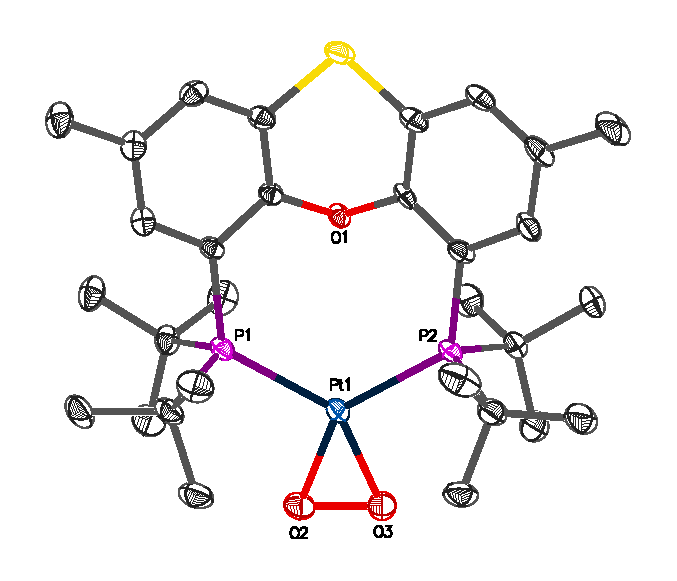
\includegraphics{../Figures/Crystalplatinumdioxygen.eps}
\caption[X-ray crystal structure of [Pt(tBu-thixantphos)(\hapto{}-\ce{O2}){]} $\cdot{}$ \ce{2C6D6}]{[Pt(tBu-thixantphos)(\hapto{}-\ce{O2})] $\cdot{}$ \ce{2C6D6}.  Hydrogen atoms and solvent molecules omitted for clarity}
\vspace{0.2cm}
\label{crystal:dioxygen}
\end{center}
\end{figure}
\vspace{0.2cm}

\begin{figure}[ht]
\begin{center}
\vspace{0.5cm}
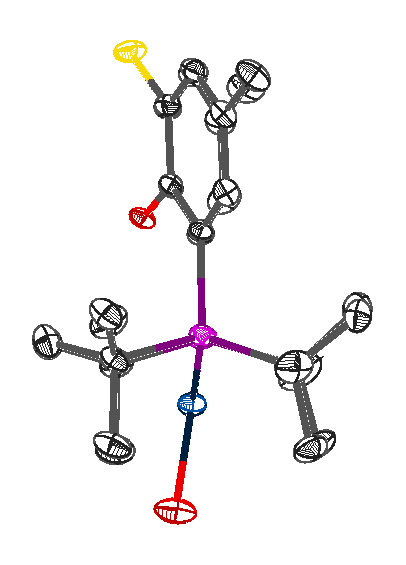
\includegraphics{../Figures/Crystalplatinumdioxygenside.eps}
\caption[X-ray crystal structure of [Pt(tBu-thixantphos)(\hapto{}-\ce{O2}){]} $\cdot{}$ \ce{2C6D6} side view]{[Pt(tBu-thixantphos)(\hapto{}-\ce{O2})] $\cdot{}$ \ce{2C6D6}, side view.  Hydrogen atoms and solvent molecules omitted for clarity}
\vspace{0.2cm}
\label{crystal:dioxygenside}
\end{center}
\end{figure}
\vspace{0.2cm}

%dioxygen
\begin{table}[ht]
\caption[Selected bond distances (\AA) and angles (\degrees) of [Pt(tBu-thixantphos)(\hapto{}-\ce{O2}){]} $\cdot{}$ \ce{2C6D6}]{Selected bond distances (\AA) and angles (\degrees) of [Pt(tBu-thixantphos)(\hapto{}-\ce{O2})}{]} $\cdot{}$ \ce{2C6D6}} 
\vspace{1em}
\label{table:crystalPtdioxygen:lengths}
\small
\begin{center}
\begin{tabular}{l l l l}
	\toprule
	\multicolumn{2}{l}{\bfseries{~Bond distances (\si{\angstrom})}} & \multicolumn{2}{c}{\bfseries{Bond angles (\degrees)}} \\
	\midrule		
	~P1-Pt		~~&~~2.3159(13)~~	&~~P1-Pt-P2			&~~117.26(5)~~	\\	
	~P2-Pt		~~&~~2.3056(13)~~	&~~P1-Pt-O2			&~~101.26(14)~~	\\
	~O1-Pt		~~&~~3.383(3)~~	&~~P2-Pt-O3			&~~100.11(13)~~	\\
	~O2-Pt		~~&~~2.024(4)~~	&~~O2-Pt-O3			&~~41.38(18)~~	\\
	~O3-Pt		~~&~~2.022(4)~~	&~~Ring 1 - Ring 2		&~~133.90(18)~~	\\
	~O1-O2		~~&~~1.429(6)~~	&~~					&~~		~~		\\
	\bottomrule{}
\end{tabular}
\end{center}
\end{table}

%dioxygen
\begin{table}[htp]
\small
\caption[Crystallographic Data and Structure Refinement of [Pt(tBu-thixantphos)(\hapto{}-\ce{O2}){]} $\cdot{}$ \ce{2C6D6}]{Crystallographic Data and Structure Refinement of [Pt(tBu-thixantphos)(\hapto{}-\ce{O2}){]} $\cdot{}$ \ce{2C6D6}} 
\vspace{1em}
\label{table:crystalPtdioxygen:data}
\small
\begin{center}
\begin{tabular}{l l}
	\toprule
	\bfseries{Empirical formula}~~& \bfseries{\ce{C42H46D12O3P2PtS}}\\
	\midrule
	Formula weight	 							& 912.04\\
	Temperature/K	 							& 120.01(10)\\
	Crystal system	 							& orthorhombic\\
	Space group	 							& Pbca\\
	a$/$\si{\angstrom}							& 17.7892(3)\\
	b$/$\si{\angstrom} 							& 15.8129(3)\\
	c$/$\si{\angstrom}							& 28.4025(5)\\
	$\alpha/$\degrees							& 90\\
	$\beta/$\degrees							& 90\\
	$\gamma/$\degrees							& 90\\
	Volume$/$\si{\angstrom\cubed}  				& 7989.6(2)\\
	Z	 									& 8\\
$\rho$\sub{calc} \si{\milli\gram}$/$\si{\milli\metre\cubed} 	& 1.516\\
\si{\metre}$/$\si{\milli\metre} 						& 3.682\\
F(000)	 									& 3664.0\\
Crystal size$/$\si{\milli\metre\cubed}	 				& 0.21 x 0.16 x 0.15\\
Radiation	 									& MoK$\alpha$ ($\lambda$ = 0.71073)\\
2$\theta$ range for data collection					& 5.348 to 65.882\degrees\\
Index ranges	 								& -27 $\leq$ h $\leq$ 26, -22 $\leq$ k $\leq$ 24, -43 $\leq$ l $\leq$ 40\\
Reflections collected	 							& 118275\\
Independent reflections	 						& 14395 [R\sub{int} = 0.0668, R\sub{sigma} = 0.0383]\\
Data$/$restraints$/$parameters					& 14395$/$0$/$456\\
Goodness-of-fit on F$^{2}$	 					& 1.101\\
Final R indexes [I$>$=2$\sigma$ (I)]	 				& R\sub{1} = 0.0638, wR\sub{2} = 0.1563\\
Final R indexes [all data]	 						& R\sub{1} = 0.0824, wR\sub{2} = 0.1718\\
Largest diff. peak/hole / e \si{\per\angstrom\cubed}		& 7.62/-3.06	\\
	\bottomrule
\end{tabular}
\end{center}
\end{table}

The crystal structure of [Pt(\tButhixantphos)\hapto{}-\ce{O2}] shows a planar geometry around the platinum with a deviation of less than 0.001 \si{\angstrom} from planarity.  The backbone of the ligand is bent to achieve a bite-angle of 117.26(5)\degrees, smaller than the calculated bite-angle of 126.98\degrees.  The bite-angle of the \tButhixantphos{} ligand in [Pt(\tButhixantphos)\hapto{}-\ce{O2}] is similar to the bite-angle in [Ag(\tButhixantphos)Cl] (116.46(8)\degrees, Table \ref{table:crystalthixantphossilverchloride:lengths}).  No interaction between the ether-bridge oxygen and the platinum is observed with a distance of 3.383(3) \si{\angstrom} between the two atoms.  All of the bond lengths and angles have typical values.  Surprisingly only four crystal structures of platinum dioxygen complexes have been reported in the CCDC, three of which are for [Pt(\hapto{}-\ce{O2}(\ce{PPh3)2}] with different solvates, (\ce{C6H6},\cite{Kashiwagi1969} \ce{CHCl3}\cite{Cheng1971} and \ce{C7H8}\cite{Cook1969}).  However, the data quality for the structure in toluene was poor.  The other reported crystal structure is for [Pt(\hapto{}-\ce{O2})(\ce{P^{t}Bu2Ph)2}]\cite{Yoshida1979}.  The Pt-O, and O-O bond lengths, and the O-Pt-O angle show little difference between the three structures (Table \ref{table:PtO2other}).  \fixme{include a table here}

\begin{table}[ht]
\caption[Selected bond distances (\AA) and angles (\degrees) of [Pt(\ce{PR3)}\hapto{}\ce{O2}{]}]{Selected bond distances (\AA) and angles (\degrees) of [Pt(\ce{PR3)}\hapto{}\ce{O2}{]}} 
\vspace{1em}
\label{table:PtO2other}
\small
\begin{center}
\begin{tabular}{l l l l l l l}
	\toprule
	~~ & \multicolumn{3}{l}{\bfseries{~Bond distances (\si{\angstrom})}} & \multicolumn{2}{c}{\bfseries{Bond angles (\degrees)}} \\
	\cmidrule(lr){2-5} \cmidrule(lr){6-7} 
	\bfseries{Compound} & \bfseries{O-O} & \bfseries{Pt-O} & \bfseries{Pt-O\fixme{prime}} & \bfseries{O-Pt-O\fixme{prime}} & \bfseries{P-Pt-P} \\
	\midrule		
	{[}Pt(\ce{P^{t}Bu2Ph)2}\hapto{}-\ce{O2}] & 1.42(2) & 2.02(1) & 2.02(1) & 41.5(5) & 113.1(2) \\
	{[}Pt(\ce{PPh3)2}\hapto{}-\ce{O2}] $\cdot$ \ce{C6H6} & 1.45(4) & 2.01(3) & 2.01(2) & 43(1) & 101.2(4) \\
	{[}Pt(\ce{PPh3)2}\hapto{}-\ce{O2}] $\cdot$ \ce{CHCl3} & 1.505(16) & 2.006(7) & 2.006(7) & 44.06(40) & 101.23(12) \\
	\bottomrule{}
\end{tabular}
\end{center}
\end{table}

The O-O bond length in [Pt(\tButhixantphos)\hapto{}-\ce{O2}] is longer than the bond length of molecular oxygen (1.21 \si{\angstrom}) indicating the reduction in the bond order upon coordination to the metal centre.  However, the bond length is slightly shorter in the \tButhixantphos{} complex than the \ce{PPh3} or \ce{P^{t}Bu2Ph} complexes.  We would expect \tButhixantphos{} to have similar electronics to \ce{P^{t}Bu2Ph}, and to be more electron donating than \ce{PPh3}.  This should mean that the O-O bond length is longer if more electron donating ligands are used as this would add to the O2 anti-bonding LUMO which should reduce the bond order and thus increase the O-O bond length.  \fixme{check if the LUMO is actually anti-bonding} However, the P-Pt-P angle is larger for \tButhixantphos{} than the other ligands.  This possibly indicates that the O-O bond length is restrained by the sterics of the \tButhixantphos{} ligand compared to in the other cases.  Hence the O-O bond length is these complexes is likely the result of a combination of both steric and electronic effects.

The tBu-thixantphos platinum alkene complexes and the 14-electron tBu-thixantphos platinum all react rapidly and irreversibly with oxygen to form the dioxygen complex \fixme{reference}.  The slow diffusion of oxygen into a benzene solution of the tBu-thixantphos platinum ethene complex resulted in crystals of the dioxygen complex suitable for X-ray diffraction whilst crystallisation of a solution of the 14-electron complex under argon resulted in crystals containing a mixture of the 14-electron and the dioxygen complex.  This is either a result of co-crystallisation or due to molecules at the surface of the crystal reacting with oxygen during mounting and data collection.  The dioxygen complex crystallised in the Pbca space group as [Pt(tBu-thixantphos)\ce{O2}] $\cdot{}$ \ce{2C6D6} (Figure \ref{crystal:dioxygen}).  
%Crystals suitable for X-ray crystallography were obtained from a benzene solution of the 14-electron complex.  The crystals were found to contain a mixture of the 14-electron and the dioxygen complex, either co-crystallised or due to the surface of the crystal reacting with oxygen during mounting and data collection.  The data quality was poor preventing anisotropic refinement.  
%
%The bite-angle of 117.25(4)\degrees{} is much smaller than the calculated bite angle \fixme{insert a reference here} due to the backbone bending and the \emph{cis} coordination in order to accommodate the dioxygen coordinating in an $\eta$\sub{2} fashion.  The oxygen-oxygen bond length is typical for platinum dioxygen complexes \fixme{refer to the crystallographic database and maybe give examples} and shows a slight lengthening upon coordination from 1.21 \si{\angstrom} in free \ce{O2} to 1.429 \si{angstrom} in the complex.  The oxygen atoms have close interactions with some of the tertiary butyl protons with the closest being 2.100 and 2.160 \si{\angstrom}.  This is within the sum of the van der waals radii (\fixme{1.20 or 1.09 \si{\angstrom}} for hydrogen and 1.52 \si{\angstrom} for oxygen).   
%
%Comparing the two crystals structures for the dioxygen and the \fixme{co-crystallised} 14-electron and dioxygen complex we can see that the dioxygen complex is very similar in both cases.  \fixme{are they in the same space group?}.   For the dioxygen complex the platinum is planar with four substituents coplanar.  In the 14-electron complex we observe a bent configuration of the platinum.  Two-coordinate platinum complexes typically form linear configurations \fixme{check CCD} so the bent configuration is likely a result of the backbone restricting the bite-angle.  
%
%\fixme{compare (overlap perhaps?) the dioxygen complexes obtained from each crystal structure}
%
%The differences between the 14-electron and the dioxygen complexes are of particular interest.  The ligands share the same sites in the disordered structure indicating that little ligand rearrangement is necessary for the dioxygen to coordinate.  The 14-electron complex has a much larger bite-angle \fixme{value?} with the platinum sitting much closer to the ether bridge.  This nicely shows how a metal centre and the presence of other ligands can influence the bite-angle of a diphosphine, these effects are not accounted for in the widely used, theoretically obtained, natural bite-angle as defined by Casey and Whiteker\cite{Casey1990} and it is notable here that we have two complexes with very similar ligand positions have bite-angles of \fixme{this and this} while the natural bite angle was calculated as \fixme{this}.

%\fixme{check the above paragraphs once the crystal structure is back from Martyn}

%======================================================================

\section{Reactions of Platinum dioxygen}

The bond length of the dioxygen molecule increases upon coordination, indicating a decrease in the bond order and strength.  As such, the oxygen molecule should be activated, and more likely to undergo reactions with small molecules, with several examples reported in the literature.  Furthermore some examples of reversible coordination of dioxygen to a palladium centre have been reported, with removal of the dioxygen ligand either by vacuum, or by substitution or reaction with other ligands.  As such we investigated the reversibility of the formation of [Pt(\tButhixantphos)\hapto{}-\ce{O2}] by vacuum and by reaction with \ce{C2H4} and investigated the activation of the oxygen ligand by reaction with various small molecules; \ce{C2H2}, \ce{H2}, CO, \ce{CO2}, \ce{NH4PF6} and 1,3,5-triaza-7-phosphaadamantane (\fixme{glossary, PTA}).

The [Pd\hapto{}-\ce{O2}(\ce{P^{t}Bu2Ph)2}] complex readily loses dioxygen under vacuum.\cite{Yoshida1979} Although [Pt\hapto{}-\ce{O2}(\ce{P^{t}Bu2Ph)2}] did not lose oxygen under the same conditions, recent work in our group has shown that [Pt\hapto{}-\ce{O2}(\ce{P^{t}Bu2Bn)}] \fixme{and Kathryn's PS ligand} can also lose oxygen.  The dioxygen ligand in [Pt(\tButhixantphos)\hapto{}-\ce{O2}] complex was not observed to dissociate despite heating the reaction under vacuum.  This result is not unexpected as the \tButhixantphos{} system is more sterically and electronically similar to \ce{P^{t}Bu2Ph} than \ce{P^{t}Bu2Bn}.  However, the larger P-Pt-P angle in the \tButhixantphos{} complex compared to \ce{P^{t}Bu2Ph} may have promoted the lose of the dioxygen ligand.  

[Pt(\tButhixantphos)\hapto{}-\ce{O2}], can be formed by reaction of [Pt(\tButhixantphos)\ce{(C2H4)}] with air.  However, bubbling ethene through an NMR sample in \ce{C6D6} for 10 minutes showed no conversion to the ethene complex.  Leaving the sample under an atmosphere of ethene for a further 48 hours showed no evidence by NMR for conversion to [Pt(\tButhixantphos)\ce{(C2H4)}] indicating that the reaction is not readily reversible, either by vacuum or by substitution of the dioxygen ligand with ethene.  

Complexes [Pd\hapto{}-\ce{O2}(\ce{P^{t}Bu2^{n}Bu)2}] and [Pd\hapto{}-\ce{O2}(\ce{PAd2^{n}Bu)2}] (Ad = 1-adamantyl) have been used as stable precatalysts for palladium catalysts formylations and alkoxycarbonylations due to their reduction to the 14-electron palladium complexes by reaction with hydrogen.\cite{Sergeev2010}  Reaction of [Pt(\tButhixantphos)\hapto{}-\ce{O2}] with hydrogen gas was attempted by bubbling the gas through the reaction mixture then sealing under an atmosphere of hydrogen.  No reaction was observed after three days, again indicating the stability of the dioxygen complex.  

Having established that the reaction of [Pt(\tButhixantphos)] with dioxygen is not readily reversible we decided to investigate the reactivity of the coordinated dioxygen ligand.  The platinum dioxygen complexes [Pt\hapto{}-\ce{O2}(\ce{PR3)2}] (\ce{PR3} = \ce{PCy3}, \ce{P^{i}Pr3}, \ce{P^{t}Bu2^{n}Bu}, \ce{P^{t}Bu2Me}, PPh3) readily react with alkynes showing 1,2-addition of the dioxygen molecule across the triple bond forming metallacyclic compounds (Scheme \ref{PtO2ethyne})\cite{Clark1978}.  Reaction of [Pt(\tButhixantphos)\hapto{}-\ce{O2}], with ethyne showed no reaction after two days at room temperature.  The absence of any reactivity may be due to the inactivity of ethyne towards dioxygen complexes (the literature examples used electron poor alkynes for this reaction), rather than any inherent stability of the dioxygen complex.  

Platinum dioxygen complexes undergo reaction with carbon monoxide to form carbonate complexes and with carbon dioxide to form peroxycarbonates.\cite{Goel1983b}  Reaction of [Pt(\tButhixantphos)(\hapto{}-\ce{O2})] with carbon dioxide again showed no reaction.  However, the reaction with carbon monoxide proved to be more complex than those previously reported, proceeding through several intermediates before forming a single stable species after seven days at room temperature.  In order to assist in identification of these intermediates, the reaction was also repeated using \carbon{}-enriched CO and the reaction was followed by \proton{}, \carbon{} and \phosphorus{} NMR spectroscopy.  However, due to the complexity of the system, little information could be gained from the \proton{} NMR spectra.  

The first step of the reaction is the expected product, with the carbon monoxide inserting into the O-O bond to form a \hapto{2}-carbonate ligand.  The \carbon{} NMR spectrum shows a peak at 167.9 ppm as a triplet (\JPC{} = 3.9 Hz) with platinum satellites (\JPtC{} = 64.4 Hz).  The \phosphorus{} NMR spectrum shows an associated peak at 15.6 ppm with platinum satellites of 4055 Hz.  Previously, this reaction has been observed with [Pt(\hapto{}-\ce{O2})(\ce{P^{t}BuPh2)2}] and [Pt(\hapto{}-\ce{O2})(\ce{P^{t}Bu2^{n}Bu)2}] which experienced upfield shifts of 9.7 and 16.3 ppm, and a decrease in the \JPtP{} = 364 and 330 Hz respectively upon reaction with CO.\cite{Goel1983b}  In the \tButhixantphos{} reaction an upfield shift of 22.8 ppm and a decrease in \JPtP{} of 433 Hz.  While the shift is greater than expected for the \tButhixantphos{} complex, the chemical shift of [Pt(\hapto{2}-\ce{CO3})(PP)] complexes with mono, or diphosphines ranges substantially (-12.0 to 58.7 ppm), ands although reported coupling constants (3377 - 3697 Hz)\cite{Goel1983b}\fixme{cite NMR book} are smaller than for [Pt(\tButhixantphos)(\hapto{2}-\ce{CO3})] (4055 Hz) we have seen throughout this chapter that the \tBuxantphos{} platinum(0) complexes typically have larger \JPtP{} values than other complexes of the same type.

The [Pt(\tButhixantphos)(\hapto{2}-\ce{CO3})] complex progresses over the course of several days into another intermediate.  This intermediate shows two different signals in the \phosphorus{} NMR spectrum at 50.5 and -38.7 ppm with platinum satellites of 1893 and 2854 Hz respectively.  This shows a loss of the symmetry of the \tButhixantphos{} ligand with the two phosphorus atoms now appearing in different environments.  The large upfield shift (48.2 ppm from the free ligand) is associated with the formation of a four-membered ring including the phosphine.\cite{Garrou1981}  In addition the phosphorus atom at 50.5 ppm has a coupling constant indicative of a \trans{} ligand with a high \trans{}-influence such as an alkyl group.  From this we can propose a \cis{} arrangement of the phosphorus atoms with metallation of one of the \tBu{} substituents on one of the \phosphorus{} atoms, creating an alkyl group \trans{} to the non-metallated phosphorus.  However for metallation to be observed we would also expect to see an upfield shift in the \proton{} NMR spectrum indicative of a platinum hydride.  No such peak was observed, instead a strongly downfield proton{} signal was observed at 17.6 ppm indicating the presence of an acidic proton.  From this information we propose the conversion of the \dento{2}-carbonate ligand into a bicarbonate using the hydrogen from the metallated \tBu{} group.  Unfortunately this complex is too short-lived to investigate the \carbon{} NMR.  

The final product is obtained by loss of carbon dioxide gas (observed in the \carbon{} NMR spectrum) from the bicarbonate complex.  The final product shows two \phosphorus{} environments; one at -49.2 ppm (\JPtP{} = 3943 Hz) and the other at 38.2 ppm (\JPtP{} = 1794 Hz).  This indicates the retainment of the \tButhixantphos{} ligand with one metallated \tBu{} group from the bicarbonate complex.  The platinum-phosphorus coupling constants show that the non-metallated phosphorus is \trans{} to the metallated \tBu{} group, while the metallated phosphorus is \trans{} to a ligand with a weak \trans{} influence.  We propose that this ligand is a hydroxyl as this would likely result from loss of \ce{CO2} from a bicarbonate, and hydroxyl ligands have low \trans{} influence.  The final product shows a signal in the \carbon{} NMR for the metallated carbon at 15.7 ppm as a doublet of doublets with coupling of 81.6 Hz to the \trans{} phosphorus and 35.6 Hz to the \cis{} phosphorus, though no platinum satellites could be observed.  The position of this peak is consistent with other platinum alkyls that occur \trans{} to phosphorus.\cite{Zayya2012, Zayya2012b}\fixme{cite Sarah's thesis}  No signal for the hydroxyl proton was observed in the \proton{} NMR spectrum which may indicate exchange with a deuterium from the solvent (\ce{CD2Cl2}.  The mass spectrum was also unable to confirm a hydroxyl ligand as a peak was observed for [M-OH\ce{]+}, as transition metal complexes typically lose weakly coordinated ligands under the harsh mass spectrometry conditions.  The overall reaction showing the intermediates is given in Scheme \ref{scheme:StBuPtO2andCO}.

\begin{scheme}[ht]
\begin{center}
\vspace{0.5cm}
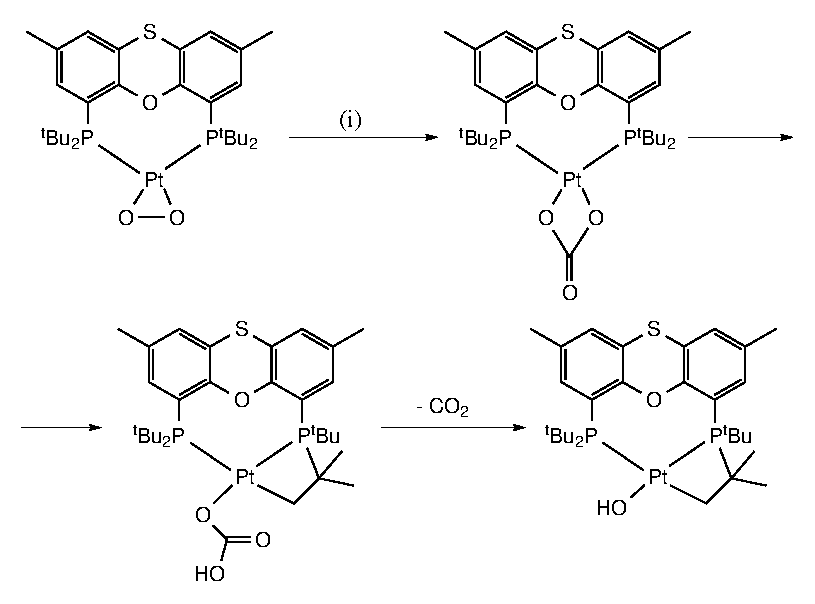
\includegraphics{../Schemes/StBuPtO2andCO.eps}
\caption[Reaction between \ce{[Pt(tBu-thixantphos)O2{]}} and CO]{Reaction between \ce{[Pt(tBu-thixantphos)O2{]}} and CO.}
\vspace{0.2cm}
\label{scheme:StBuPtO2andCO}
\end{center}
\end{scheme}
\vspace{0.2cm}

%Intermediate \fixme{give a reference} then loses carbon dioxide (enriched when using \carbon{}O) to give the final product \fixme{reference}.  The final product is asymmetric and retains the metallacycle from the \fixme{reference} previous compound.  The two phosphines appear at 38.2 (\JPtP{} = 1794 Hz) and -49.6 ppm (\JPtP{} = 3943 Hz).  The small coupling constant for the non-metallated carbon indicates that it is trans to a ligand with a strong trans influence, in this case the metalled t-butyl group.  The metalled phosphorus shows the significant downfield shift expected for metallation.  The identity of the final ligand has not been conclusively identified.  The large coupling constant for the metallated carbon suggests a ligand with a weak trans influence such as a halide or an oxygen donor.  The mass spec gives a signal for [M-L]\textsuperscript{+} so is of little assistance.  A hydroxyl ligand is the likely by-product from the loss of \ce{CO2} from fix me{reference}, and we would expect that a hydroxyl may well exchange with deuterium and be broad in the \proton{} NMR thus explaining the absence of the signal.  

The final two structures are particularly note-worthy due to the \cis-coordination of the phosphines.  Such sterically bulky ligands show a distinct preference for trans-coordination (as we will see in \fixme{reference to platinum(II) stuff}).  The metallacyclobutane must be cis, however the ligand could still maintain a trans coordination.  It is likely that the coordination plane is distorted and the phosphines are not perfectly 90\degrees{} thus allowing for pseudo-cis coordination.  In addition the metallation of the \tBu{} may hold that part of the molecule in a particular geometry resulting in less steric hindrance for the other phosphine.  

Despite such unexpected chemistry with CO, [Pt(\tButhixantphos)(\hapto{}-\ce{O2})] show a distinct stability to other small molecules.  No reaction with ammonium hexafluorophosphate or with methane.  However, a straightforward reaction does occur with PTA.  PTA is a phosphine ligand with a very small cone angle making it an ideal choice to react with the sterically restrained system.  Reaction with PTA showed immediate reaction producing peaks in the \phosphorus{} NMR spectrum at 9.5 and -74.1 ppm (\JPtP{} = 3562 Hz).  The peak at 9.5 ppm did not show any coupling to platinum and is consistent with uncoordinated \tButhixantphos{} ligand.  The peak at -74.1 ppm is consistent with the literature reported [Pt(PTA\ce{)4}] complex.  The \proton{} and \carbon{} NMR data confirm these assignments.  No intermediates were observed due to the speed of the reaction.  This suggests that PTA is able to displace both the dioxygen and the \tButhixantphos{} ligand from the platinum, and thus is too reactive to gain any insight into the activation of the dioxygen moiety.  
%
%
%
%In order to investigate the activation of the oxygen that occurred upon coordination a number of reactions were carried with the dioxygen complex and other small molecules.  It is unreactive towards ethene and ethyne.  The reaction with 1,3,5-triaza-7-phosphaadamantane (PTA) yielded uncoordinated tBu-thixantphos and \ce{[Pt(PTA)4]} with consistent spectroscopic data to previous reports.\fixme{citation} 
%
%A number of palladium dioxygen complexes have been reported to be reduced to palladium(0) 14-electron complexes using hydrogen, either as the pure gas or as a mixture with carbon monoxide such as in formylations and alkoxy carbonylations.\cite{Sergeev2010}  However, metal dioxygen complexes have also been reported as reacting rapidly with carbon monoxide yielding a metal carbonate.\cite{Goel1983b}  This indicates that in general palladium dioxygen complexes preferentially react with hydrogen rather than carbon monoxide.  As such, we decided to investigate the reactivity of the platinum dioxygen complexes with both carbon monoxide and with hydrogen.  \fixme{I should actually react it with hydrogen at some point...}
%  
%The dioxygen complex \fixme{reference} reacts with carbon monoxide and forms a series of intermediates before a stable final product is observed (Scheme \ref{scheme:StBuPtO2andCO}).  The reaction was carried out with enriched \textsuperscript{13}CO and a number of intermediates were able to be identified.  The first product is the expected carbonate complex \fixme{reference?} \ce{[Pt(tBu-thixantphos)CO3]} with the carbonate appearing in the \carbon{} NMR spectrum at 167.85 ppm (t, 3.9 Hz, \JPtC{} = 64.4 Hz).  This is associated with a single environment in the \phosphorus{} NMR spectrum at 15.6 ppm with \JPtP{} = 4055.4 Hz.  
%
%
%
%Unlike previously reported carbonate complexes \ce{[Pt(tBu-thixantphos)CO3]} reacts further. 
%A down-field peak is observed in the proton NMR at 17.6 ppm indicating the presence of an acidic proton.  There are also two phosphorus peaks at 50.5 ppm and -38.7 ppm with satellites of 1893 and 2854 respectively.  The upfield shift of one phosphorus is commonly associated with metallation of a tertiary butyl group.\cite{Garrou1981}  Based on this data intemediate \fixme{reference} is proposed. 
%
%
%
%\fixme{check if metallacycles can include phosphines or just carbons and metals}



%======================================================================

\section{Reactions with Palladium(0) Precursors}

Platinum complexes are frequently synthesised as models for the analogous palladium species as they are frequently more stable, and the presence of \Pt{} allows for additional information in the NMR spectra which can be useful in characterisation.  However, palladium complexes are of particular interest due to their use in a wide range of catalytic processes.  These systems often involve both palladium(0) and palladium(II) complexes.  As such, we investigated the reactivity of the \tBuxantphos{} ligands towards palladium(0) starting materials.  All reactions in discussed in this section were carried out on an NMR scale.  

Initial investigations focussed on the reaction of \tButhixantphos{} with palladium(0) starting materials that are commonly used in catalysis.  Allyl-cyclopentadiene palladium(0) frequently reacts in catalytic reactions as the reductive elimination of the allyl and cyclopentadiene ligands can form free coordination sites for the substrates to coordinate to.  Reaction of \tButhixantphos{} with  [Pd(\ce{C3H5})Cp] in \ce{C6D6} was slow.  After 24 hours at room temperature no changes in the NMR spectra were observed.  After 48 hours at 50 \degC, the reaction showed no unreacted \tButhixantphos{} in the \phosphorus{} NMR spectrum.  However, the \phosphorus{} and \proton{} NMR spectra showed a number of different products which were unable to be separated or analysed further.

[\ce{Pd2(dba)3}] (\fixme{glossary, dba = dibenzylideneacetone}), is another common palladium(0) compound used as a precatalyst.  Reaction of \tButhixantphos{} with [\ce{Pd2(dba)3}] also generated a mixture.   However, a single major product was observed at 40.0 ppm in the \phosphorus{} NMR spectrum (\ce{C6D6}), after heating at 40\degC{} for four days.  The major product accounted for 67\% of the \phosphorus{} NMR signals while uncoordinated \tButhixantphos{} accounted for 17\% of the reaction mixture.  The species was not the [Pd(\tButhixantphos)] as this will be discussed shortly.  However, the product was unable to be isolated from the reaction mixture and the presence of large amounts of uncoordinated dba hampered the further characterisation of this species.  It is possible that the species was [Pd(\tButhixantphos)(dba)] although little evidence to support this could be obtained.  

Platinum alkene complexes make excellent starting materials for the formation of platinum(0) complexes, particularly the air-stable solids [Pt(COD\ce{)2}] and [Pt(nb\ce{)3}].  Although [Pt(\ce{C2H4)3]} is only stable under an ethene atmosphere it is readily synthesised \fixme{in situ} \emph{via} reaction of ethene with [Pt(COD\ce{)2}].  Unfortunately the corresponding palladium complexes are typically unstable at room temperature in solution and not practical to be used as starting materials.\cite{Green1977}  However, given the slow reactivity of \tButhixantphos{} with [Pd(\ce{C3H5})Cp] and [\ce{Pd2(dba)3}], coupled with the desire to investigate the analogue of the platinum alkene complexes discussed earlier, we decided to investigate the reactivity of\tButhixantphos{} towards [Pd(nb\ce{)3}].  Tris-norbornenepalladium, like other palladium alkenes is unstable in solution, with large amount of degradation observed at room temperature.  However, the amount of degradation can be reduced by addition of excess norbornene to the reactions.  

Reaction of \tButhixantphos{} with [Pd(nb\ce{)3}] was rapid compared to the other palladium(0) starting materials, going to completion in less than one hour forming a single complex.  As such the reaction was also carried out with \tBusixantphos{} and \tBuxantphos{}.  For \tBuxantphos{} the reaction was also complex in under one hour, while reaction with \tBusixantphos{} showed only 43.4\% product (the remainder being free ligand) after 24 hours.  The reaction continued to be followed by NMR and after 48 hours no further change was observed.  However, after five months at room temperature the reaction had progressed to 68\% complex indicating that the lack of reactivity was not necessarily due to degradation of the [Pd(nb\ce{)3}].  

Both \tButhixantphos{} and \tBusixantphos{} formed only one species, while \tBuxantphos{} formed a mixture though one complex was the major product.  The products appear at 41.9-42.9 ppm in the \phosphorus{} NMR spectrum.  Given the similarity in the \phosphorus{} chemical shift and the inability to isolate the \tBusixantphos{} and \tBuxantphos{} complexes, the \tButhixantphos{} complex was the only product explored in depth.  Once the product is formed the norbornene was able to be removed under vacuum with no degradation of the resulting complex.  The complex displays no resonances in the \proton{} and \carbon{} NMR spectra apart from those corresponding to a coordinated \tButhixantphos{} ligand.  Hence the complex formed in these reactions is [Pd(\tBuxantphos)] (Scheme \ref{scheme:Pd14}).  

Given the presence of excess norbornene and the mixtures that were observed upon reaction of the \tBuxantphos{} ligands with [Pt(nb\ce{)3}], we might expect the presence of a [Pd(\tBuxantphos)(nb)] complex.  However, alkenes coordinate more strongly to platinum than palladium, meaning that even the excess norbornene is insufficient to promote the formation of a norbornene complex.  Furthermore the \proton{} and \carbon{} NMR spectra of [Pd(\tButhixantphos)] clearly show virtual triplet signals for the \tBu{} environments.  This is consistent with the \trans{} coordination of the phosphorus atoms, and the absence of any alkene ligand.  

\subsection{Reaction of [Pd(\tButhixantphos)] with oxygen}

As discussed previously the [Pt(\tButhixantphos)] complex is highly reactive and reacts rapidly and irreversibly with dioxygen to form [Pt(\hapto{}-\ce{O2}(\tButhixantphos)].  However, previous examples  have indicated that the coordination of dioxygen to palladium is frequently reversible even if the platinum analogue is not.\cite{Yoshida1979}  Reaction of [Pd(\tButhixantphos)] with oxygen occurs rapidly forming a green [Pd(\hapto{}-\ce{O2}(\tButhixantphos)] complex.  The \phosphorus{} NMR spectrum shows a smaller change in chemical shift than is observed with the platinum analogue (9.1 compared to 40.2 ppm) and the shift is downfield rather than upfield in the platinum case.  This is likely due to marked differences in the 14-electron complexes rather than the dioxygen complexes as [Pt(\tButhixantphos)] appears at 78.6 ppm while [Pd(\tButhixantphos)] is at 42.9 ppm.  The \tBu{} signals in the \proton{} and \carbon{} NMR spectra of [Pd(\tButhixantphos)] now appear as doublets indicating the loss of the \trans{} arrangement of the phosphorus atoms which results in the virtual triplet signals.  

The reaction of [Pd(\tButhixantphos)] with dioxygen was observed to be readily reversible.  Simply removed the solvent from the NMR sample under vacuum for a few minutes was sufficient for the dioxygen to dissociate and undergo complete reversion to [Pd(\tButhixantphos)].  This is consistent with the literature which indicates that coordination of dioxygen to palladium complexes is typically reversible.  This may be due to the reduced back-bonding of palladium compared to platinum, which results in less activation of the O-O bond upon coordination, such that on palladium the dioxygen is more like a neutral \ce{O2} ligand while on platinum the dioxygen become more like a peroxy \ce{O2^{2-}}.  

%Attempts to synthesise palladium(0) complexes were much less successful than the work with platinum(0).  Reaction between \ce{Pd2dba3} and tBu-thixantphos resulted in a single complex which showed similarities to the platinum xantphos dioxygen complexes that formed from the 14-electron complex.  A single product at 40.0 ppm in the \phosphorus{} NMR spectrum was observed and did not appear to have any associated dba.  However, the was unable to be separated from the uncoordinated dibenzylideneactone by-product. \fixme{my Pt(O2) complex is insoluble in benzene and dba probably is soluble so maybe washing with some toluene might be enough? Or crystallisation from toluene}
%
%Cyclopentadiene palladium allyl is often used as a palladium(0) precursor in catalytic reactions as the reductive elimination of the cyclopentadiene and the allyl generates a palladium(0) and an inert \fixme{C8H8?} alkyl which is generally unreactive towards the catalyst.  Reaction between cyclopentadiene palladium allyl and tBu-thixantphos was attempted with little success.  A number of products were observed with peaks appearing at 33.5, 42.9 and 51.9 ppm in the \phosphorus{} NMR spectrum in addition to the dioxygen complex which forms over times at 40.0 ppm.  The major product is the broad signal at 42.9 ppm which may be an allyl complex or something?
%
%The \carbon{} NMR spectrum showed signals at 147.2 and 145.1 ppm which have previously been seen with this ligand for the proton adjacent to the phosphine selenide.  This significant shift is a result of close proximity to a heavy atom so it may be that a very unusual coordination has formed including perhaps dimers or oligomers?  It is also possible that there may be an allyl or something strange forming \fixme{check for free cp} perhaps some sort of propene structure?
%
%An alternative route to palladium(0) could include the reaction with tris-(norbornene)palladium which would be an exact analogue of the successful reaction with tris-(norbornene) platinum.  Another attempt could be via the reduction of the relatively easy to synthesise dichloropalladium tBu-xantphos complexes.  However reduction of palladium dichlorides requires a cis-coordination of the chlorides if this is not the case then the chlorides are often substituted for hydride ligands.\fixme{try this and see what happens with [Pd(tBu-thixantphos)Cl]}.  In this case however, due to the lability of palladium and one of the chloride ligands it may be that it can reorganise to a pseudo-cis configuration for the reduction or I may form a dihydride.  It is also possible that this is atmosphere dependent and that doing the reaction in the air may result in the Pd(0) dioxygen complex.  



%======================================================================

\section{Computational Results}

As we have seen throughout this chapter the chemistry of these complexes appears subtle, forming mixtures products and some readily reversible systems.  However, a number of the complexes were unable to be isolated and fully characterised.  As such, we have investigated the conversion of the [M(\tBuxantphos)] complexes to [M(\tBuxantphos)(nb)] or [M(\tBuxantphos)(\hapto{}-\ce{O2})] (M = Pd, Pt) using DFT.  Structural models of the complexes were optimised and their vibrational frequencies calculates using a B3LYP functional,\cite{Becke1993, Lee1988, Vosko1980, Stephens1994} with the def2-TZVP basis set.\cite{Andrae1990, Weigend2005}  Selected bond lengths and angles are given in Tables \ref{DFT:14electron}, \ref{DFT:nb} and \ref{DFT:O2} for [M(\tBuxantphos)], [M(\tBuxantphos)(nb)] and [M(\tBuxantphos)(\hapto{}-\ce{O2})] respectively.  

\fixme{tables and discussion}

The Gibbs free energy for each of the complexes were also calculated and the values of $\Delta$G for reaction of the 14-electron complexes with norbornene  were calculated (Tables \ref{DFT:nbenergy}).  Reaction of the [Pt(\tBuxantphos)] complexes with norbornene results in a positive $\Delta$G value indicating that the reaction would not occur spontaneously and the 14-electron complex is the lower energy system.  This is consistent with the experimental results for the palladium reaction.  However, in the platinum system mixtures of the norbornene and the 14-electron complexes were observed for both \tBusixantphos{} and \tButhixantphos.  In the case of \tBuxantphos{} the 14-electron complex was formed initially but this converted to [Pt(\tBuxantphosk)H\ce{]+}.  This hydride complex is likely the result of the 14-electron complex undergoing reaction with another component of the system.  Hence although the [Pt(PP)] is formed as the major product experimentally an equilibrium with the norbornene complex is likely present.  The values of $\Delta$G do not take into account the activation energy of the system.  It is likely given that norbornene coordinates more strongly to platinum, that although the 14-electron complex is thermodynamically favoured the kinetic product is the norbornene complex, which is likely an intermediate on the way to the 14-electron complex.  

\begin{sidewaystable}[htb]
\caption[Gibbs free energies calculated for reaction of [M(\tBuxantphos){]} with norbornene]{Gibbs free energies calculated for reaction of [M(\tBuxantphos)] with norbornene (M = Pd, Pt).  Norbornene G = -715998.2 \si{\kilo\joule\per\mole}}
\vspace{1em}
\label{DFT:nbenergy}
\small
\begin{center}
\begin{tabular}{l c c c c c c}
	\toprule
	~\bfseries{PP} & {[}Pd(PP)] & {[}Pd(PP)(nb)] & Pd $\Delta$G & {[}Pt(PP)] & {[}Pt(PP)(nb)] & Pt $\Delta$G \\
	\midrule		
	~\tBuSixantphos	& -6163451.1	& -6879350.9 & 98.4 & -6140995.8 & -6856897.4 & 96.6 \\
	~\tBuThixantphos	& -6445645.2	& -7161551.4 & 92.1 & -6423187.2 & -7139098.3 & 87.1 \\
	~\tBuXantphos{}	& -5503258.5	& -6219169.0 & 87.8 & -5480799.2 & -6196709.7 & 87.7 \\
	\bottomrule{}
\end{tabular}
\end{center}
\end{sidewaystable}

The values for the Gibbs free energies of the [M(\hapto{}-\ce{O2})(PP)] complexes were also calculated together with the $\Delta$G values for their formation from the [M(PP)] complexes (Table \ref{DFT:O2energy}).  All of the $\Delta$G values are negative, indicating that the dioxygen complex is the thermodynamically favoured product.  The $\Delta$G values for the palladium complexes are more negative than the platinum ones.  This suggests that the palladium complexes should be more stable than the platinum system to reversibility.  However, this was not observed experimentally for the \tButhixantphos{} system where the platinum dioxygen complex was very stable and the palladium dioxygen complex readily converted to the 14-electron.  From Table \ref{DFT:O2} we can see that the P-M-P angle is consistently larger in the palladium complexes than the platinum, while the O-O bond length is smaller for the palladium complexes.  This indicates that the dioxygen ligand is more sterically hindered on the palladium and the O-O bond is less activated meaning it is more close to free \ce{O2} and thus is more likely to dissociate.  

\begin{sidewaystable}[htb]
\caption[Gibbs free energies calculated for reaction of [M(\tBuxantphos){]} with oxygen]{Gibbs free energies calculated for reaction of [M(\tBuxantphos)] with oxygen (M = Pd, Pt).  Oxygen G = -394857.8 \si{\kilo\joule\per\mole}}
\vspace{1em}
\label{DFT:O2energy}
\small
\begin{center}
\begin{tabular}{l c c c c c c}
	\toprule
	~\bfseries{PP} & {[}Pd(PP)] & {[}Pd(\hapto{}-\ce{O2})(PP)] & Pd $\Delta$G & {[}Pt(PP)] & {[}Pt(\hapto{}-\ce{O2})(\tBuxantphos)] & Pt $\Delta$G \\
	\midrule		
	~\tBuSixantphos	& -6163451.1	& -6558323.8 & -14.8 & -6140995.8 & -6535862.4 & -8.8 \\
	~\tBuThixantphos	& -6445645.2	& -6840520.9 & -17.8 & -6423187.2 & -6818062.4 & -17.4 \\
	~\tBuXantphos{}	& -5503258.5	& -5898134.9 & -18.6 & -5480799.2 & -5875674.2 & -17.2 \\
	\bottomrule{}
\end{tabular}
\end{center}
\end{sidewaystable}
%
%\begin{table}[htb]
%\caption[Bond lengths and angles for [M(\tBuxantphos){]}]{Bond lengths and angles for [M(\tBuxantphos){]}}
%\vspace{1em}
%\label{DFT:14electron}
%\small
%\begin{center}
%\begin{tabular}{l c c c}
%	\toprule
%	~\bfseries{PP} & Pt-P & Pt-P & P-Pt-P \\
%	\midrule		
%	~\tBuSixantphos	
%	~\tBuThixantphos	
%	~\tBuXantphos{}	
%	\bottomrule{}
%\end{tabular}
%\end{center}
%\end{table}
%
%\begin{sidewaystable}[htb]
%\caption[Bond lengths and angles for [M(\tBuxantphos)(nb){]}]{Bond lengths and angles for [M(\tBuxantphos)(nb){]}}
%\vspace{1em}
%\label{DFT:nb}
%\small
%\begin{center}
%\begin{tabular}{l c c c c c c c}
%	\toprule
%	~\bfseries{PP} & Pt-P & Pt-P & Pt-C & Pt-C & C-C & P-Pt-P & C-Pt-C \\
%	\midrule		
%	~\tBuSixantphos	
%	~\tBuThixantphos	
%	~\tBuXantphos{}	
%	\bottomrule{}
%\end{tabular}
%\end{center}
%\end{sidewaystable}
%
\begin{sidewaystable}[htb]
\caption[Bond lengths and angles for [M(\tBuxantphos)(\hapto{}-\ce{O2}){]}]{Bond lengths and angles for [M(\tBuxantphos)(\hapto{}-\ce{O2}){]}}
\vspace{1em}
\label{DFT:O2}
\small
\begin{center}
\begin{tabular}{l c c c c}
	\toprule
	~\bfseries{PP} & P-Pt-P & P-Pd-P & O-O (Pt) & O-O (Pd) \\
	\midrule		
	~\tBuSixantphos	115.3 & 118.7 & 1.4083 & 1.3714\\
	~\tBuThixantphos	116.8 & 118.6 & 1.4078 & 1.3710\\
	~\tBuXantphos{}	117.2 & 119.6 & 1.4070 & 1.3705\\
	\bottomrule{}
\end{tabular}
\end{center}
\end{sidewaystable}






%======================================================================

\section{Summary and Conclusions}


